\section{AHTR One-Third Assembly Optimization Results Discussion}
\label{sec:assem-discussion}
Chapter \ref{chap:ahtr-plank-opt-results} characterized the \gls{AHTR} plank model's 
reactor optimization objectives' driving factors and their relationship with 
one another. 
This section utilizes the previous \gls{AHTR} plank characterizations and conducts 
a deep-dive to verify if the same driving factors apply to the \gls{AHTR} one-third 
assembly model's optimization objectives. 
I also analyze how their combined effects result in the optimal reactor models found by 
the multi-objective optimization simulations. 

\subsection{Discussion: Minimize $PF_{total}$ Objective}
\label{sec:assem-discussion-pf}
\paragraph{Simulation a-1a}
In Section \ref{sec:assem-1-obj-pf}'s simulation a-1a, I conducted a single-objective 
optimization simulation to minimize the one-third assembly's total fuel packing fraction 
($PF_{total}$) by varying $PF_{total}$ and TRISO distribution. 
\gls{ROLLO} found that an \gls{AHTR} one-third assembly model with 
the most-minimized $PF_{total}$ has a $PF_{total}= 0.0559$ and an oscillating TRISO 
distribution along the both the x-axis and y-axis, and a packing fraction standard 
deviation of $0.04$ across the one-third assembly (Figure \ref{fig:assem-obj-1-pf-final}).

Section \ref{sec:plank-discussion-pf} concluded that for the \gls{AHTR} plank model, 
the minimize $PF_{total}$ objective is driven by maximizing the total fission reaction 
rates. 
I ran a simulation for constant $PF_{total} = 0.0559$ TRISO distribution and compared its 
fission reaction rate with simulation a-1a's oscillating TRISO distribution that 
most-minimized $PF_{total}$. 
Figure \ref{fig:assem-0.0559-comparison} shows the TRISO distributions for the two 
compared reactor models: Figure \ref{fig:assem-obj-1-pf-final}'s most-minimized 
$PF_{total}$ and the constant $PF_{total} = 0.0559$. 
\begin{figure}[htbp!]
    \centering
    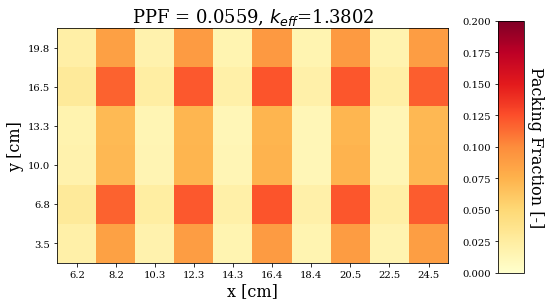
\includegraphics[width=0.49\linewidth]{assem-0.0559-most-minimized.png} 
    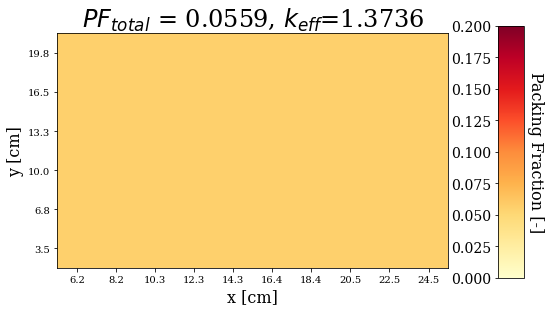
\includegraphics[width=0.49\linewidth]{assem-0.0559-flat.png} 
    \caption{Simulation a-1a's most-minimized $PF_{total}$ TRISO distribution 
    (oscillating TRISO distribution) from Figure \ref{fig:assem-obj-1-pf} (left) and the 
    constant $PF_{total} = 0.0559$ TRISO distribution (right).}
    \label{fig:assem-0.0559-comparison}
\end{figure}
The reactor model with the most-minimized $PF_{total}$ has $k_{eff}=1.3802$ and 
the reactor model with constant TRISO distribution has $k_{eff}=1.3736$.

Table \ref{tab:a-1a-fission-comparison} compares the total fission reaction rate 
(OpenMC's \texttt{fission} tally) between the most-minimized $PF_{total}$ TRISO 
distribution and a constant $PF_{total} = 0.0559$ TRISO distribution (both shown in 
Figure \ref{fig:assem-0.0559-comparison}).
\begin{table}[htbp!]
    \centering
    \onehalfspacing
    \caption{Total fission reaction rate comparison between simulation a-1a's 
    most-minimized $PF_{total}$ TRISO distribution and a constant $PF_{total} = 0.0559$ 
    TRISO distribution. Both distributions shown in Figure 
    \ref{fig:assem-0.0559-comparison}.}
	\label{tab:a-1a-fission-comparison}
    \footnotesize
    \begin{tabular}{p{1.5cm}lp{3.7cm}p{4cm}p{2.5cm}}
    \hline
    \textbf{Energy Group} & 
    \textbf{$\%$ of Total} &
    \textbf{Most-minimized $PF_{total}$ Fission \newline [reactions/src]} & 
    \textbf{Flat $PF_{total}$ Fission [reactions/src]} & 
    \textbf{$\%$ Fission \newline Difference}\\
    \hline 
    1 & 00.28 & 0.00165 & 0.00162 & \Plus2.01 \\
    2 & 01.56 & 0.00886 & 0.00884 & \Plus0.21 \\
    3 & 01.51 & 0.00854 & 0.00852 & \Plus0.23 \\
    4 & 96.63 & 0.54813 & 0.54465 & \Plus0.63 \\
    Total & - & 0.52998 & 0.52656 & \Plus0.65 \\
    \hline
    \end{tabular}
\end{table}
The most-minimized $PF_{total}$ TRISO distribution has $0.65\%$ higher  
total fission reaction rate than the constant $PF_{total} = 0.0559$ TRISO distribution. 
For the same $PF_{total}$, the oscillating TRISO distribution enabled a 
660pcm higher in $k_{eff}$ compared to the constant TRISO distribution. 
Therefore, the minimize $PF_{total}$ objective is driven by maximizing the total fission 
reaction rates to find a reactor model with a lower $PF_{total}$ that meets $k_{eff}$ 
constraints. 

\paragraph{Simulation a-1d}
In Section \ref{sec:assem-1-obj-pf}'s simulation a-1d, I conducted a single-objective 
optimization simulation to minimize total fuel packing fraction ($PF_{total}$) by 
varying $PF_{total}$ and coolant channel shape. 
In simulation a-1d, \gls{ROLLO} found that there is no correlation 
between $PF_{total}$ and coolant channel shape (demonstrated in Figure 
\ref{fig:a-1d}). 

\paragraph{Summary}
I verified that the minimize $PF_{total}$ objective for the \gls{AHTR} one-third 
assembly model is also driven by maximizing the total fission reaction rates. 
The minimize $PF_{total}$ objective influences oscillations in the TRISO disribution.
The objective has no correlation with coolant channel shape input parameter. 

\subsection{Discussion: Minimize $T_{max}$ Objective}
\label{sec:assem-discussion-temp}
\paragraph{Simulation a-1b}
In Section \ref{sec:assem-1-obj-temp}'s simulation a-1b, I conducted a single-objective 
optimization simulation to minimize the one-third assembly's maximum temperature 
($T_{max}$) by varying TRISO distribution. 
In simulation a-1b, \gls{ROLLO} found that for $PF_{total}$ = 0.06, the reactor model 
with the most-minimized $T_{max}$ has a $T_{max} = 1161.28K$ with an almost constant 
TRISO distribution (Figure \ref{fig:assem-obj-1-temp-final}). 

\paragraph{Simulation a-1e}
In Section \ref{sec:assem-1-obj-temp}'s simulation a-1e, I conducted a single-objective 
optimization simulation to minimize the one-third assembly's maximum temperature 
($T_{max}$) by varying coolant channel shape. 
In simulation a-1e, \gls{ROLLO} found that there is a negative linear correlation 
between the one-third assembly's $T_{max}$ and $r_1$ and $r_5$, but no correlation with 
$r_2$, $r_3$, and $r_4$, shown in Figure \ref{fig:a-1e}. 

Figures \ref{fig:a-1e-temp-distribution-2d} and \ref{fig:a-1e-temp-distribution-centerline}
show the 2D temperature distribution and centerline temperature for simulation a-1e's 
one-third assembly model with the most-minimized $T_{max}$ (Figure 
\ref{fig:assem-obj-1-temp-most-minimized-coolant}). 
\begin{figure}[htbp!]
    \begin{subfigure}{\textwidth}
        \centering
        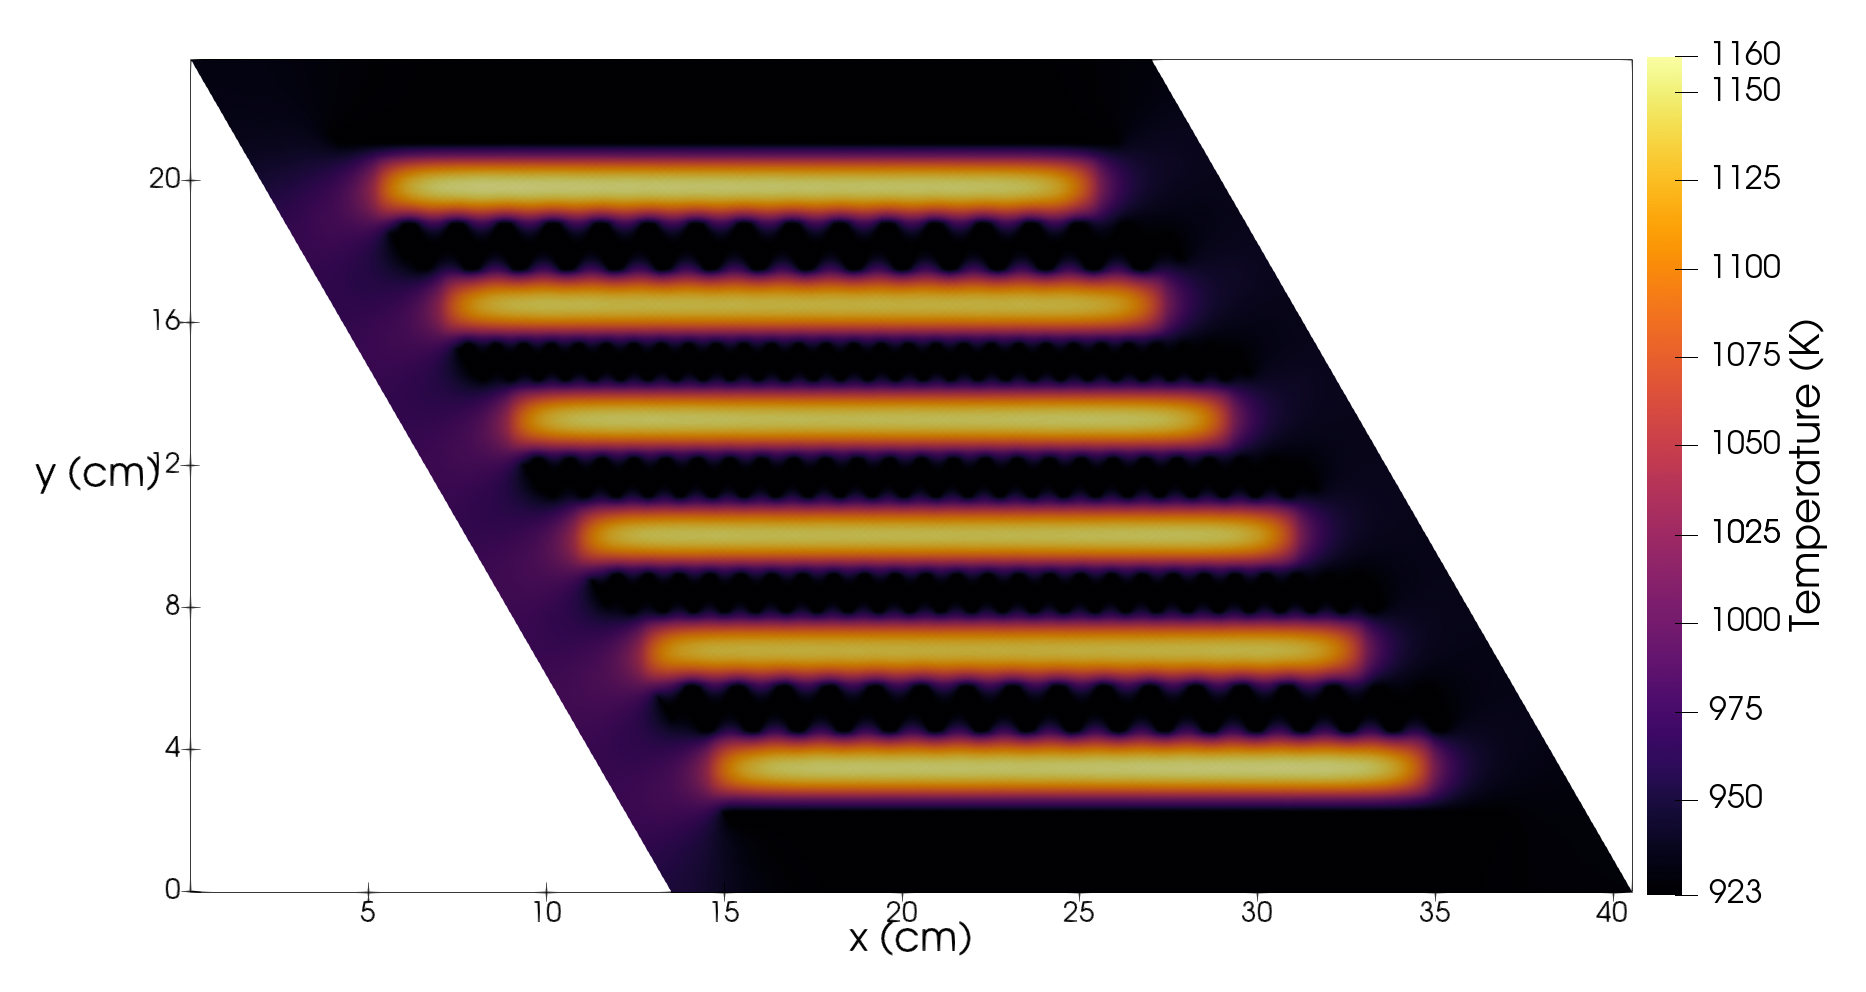
\includegraphics[width=\linewidth]{a-1e-temp-distribution-2d.png}
        \caption{2D temperature distribution.}
        \label{fig:a-1e-temp-distribution-2d} 
    \end{subfigure}
    \begin{subfigure}{\textwidth}
        \centering
        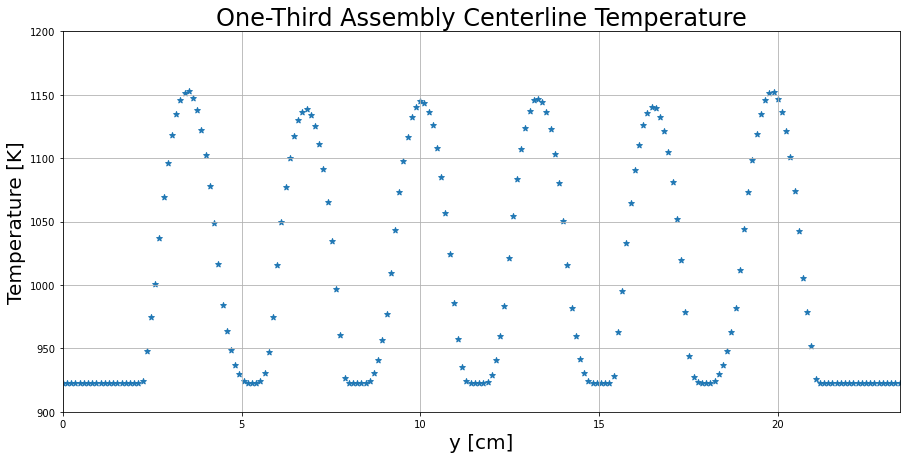
\includegraphics[width=\linewidth]{a-1e-temp-distribution-centerline.png}
        \caption{Centerline temperature. AHTR assembly's centerline is the white line 
        in Figure \ref{fig:ahtr-assem-verification}.}
        \label{fig:a-1e-temp-distribution-centerline} 
    \end{subfigure}
    \caption{Simulation a-1e's most-minimized $T_{max}$ one-third assembly reactor 
    model's temperature distribution.}
    \label{fig:a-1e-temp-distribution}
\end{figure}
Figure \ref{fig:a-1e-temp-distribution} demonstrates that for simulation a-1e's 
most-minimized $T_{max}$ reactor model, the temperature peaks in top and bottom 
graphite planks. 
$r_1$ and $r_5$ control the coolant channel shape of the \gls{FLiBe} channels closest 
to the top and bottom graphite planks. 
This explains why \gls{ROLLO} found a negative linear correlation 
between the one-third assembly's $T_{max}$ and $r_1$ and $r_5$. 
To minimize maximum one-third assembly temperature, \gls{ROLLO} maximized
$r_1$ and $r_5$ to enable enhanced cooling in the top and bottom graphite planks. 
Thus, depending on the temperature distribution in a one-third assembly, the \gls{FLiBe} 
channels (corresponding to $r_1, r_2, r_3, r_4, r_5$) closest to the temperature peaks 
will be most important to minimizing $T_{max}$. 

Comparison of simulation a-1b and a-1e's results in 
Figures \ref{fig:assem-obj-1-temp-evol} and \ref{fig:a-1e-evol} 
show that coolant channel shape variation does not have as high of an impact on 
$T_{max}$ as \gls{TRISO} distribution variation: the average $T_{max}$ due to 
\gls{TRISO} variation decreased by $\sim150K$ over 3 generations, while average 
$T_{max}$ due to coolant channel shape variation only decreased by $\sim10K$ over 
3 generations. 

\paragraph{Summary}
I verified that similar to the \gls{AHTR} plank model, a flatter TRISO distribution 
minimizes the one-third assembly's $T_{max}$. 
For the one-third assembly, the FLiBe channels (corresponding to $r_1, r_2, r_3, r_4, 
r_5$) closest to the temperature peaks will be most important to minimizing maximum
one-third assembly temperature, and thus, will show a negative correlation with 
$T_{max}$. 
The results from simulation a-1b and a-1e suggest that the minimize $T_{max}$ objective 
is more influenced by the TRISO distribution than the coolant channel shape. 

\subsection{Discussion: Minimize $PPF_{fuel}$ Objective}
\label{sec:assem-discussion-ppf}
\paragraph{Simulation a-1c}
In Section \ref{sec:assem-1-obj-ppf}'s simulation a-1c, I conducted a single-objective 
optimization simulation to minimize fuel-normalized power peaking factor ($PPF_{fuel}$) 
by varying TRISO distribution. 
In simulation a-1c, \gls{ROLLO} found that for $PF_{total}$ = 0.06, the reactor model 
with the most-minimized $PPF_{fuel}$ has a $PPF_{fuel} = 1.0872$, an oscillating 
TRISO distribution along the x-axis, and a packing fraction standard deviation of 
$0.017$ across the one-third assembly (Figure \ref{fig:assem-obj-1-ppf-final}). 

Section \ref{sec:plank-discussion-pf} concluded that for the \gls{AHTR} plank 
model, the minimize $PPF_{fuel}$ objective is driven by flattening thermal 
(Group 4) flux distribution. 
I compare the flux distributions for simulation a-1c's most-minimized $PPF_{fuel}$ 
reactor model ($PPF_{fuel} = 1.0872$) and the reactor model in simulation a-1c's 
final generation with the highest $PPF_{fuel} = 1.2431$. 
Figure \ref{fig:a-1c-ppf-triso-comparison} shows the TRISO distributions for the 
compared reactor models. 
\begin{figure}[htbp!]
    \centering
    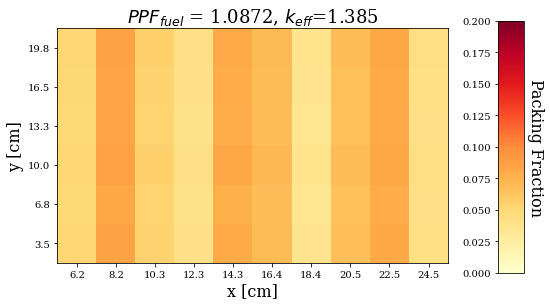
\includegraphics[width=0.49\linewidth]{a-1c-ppf-triso-comparison-most-minimized.png} 
    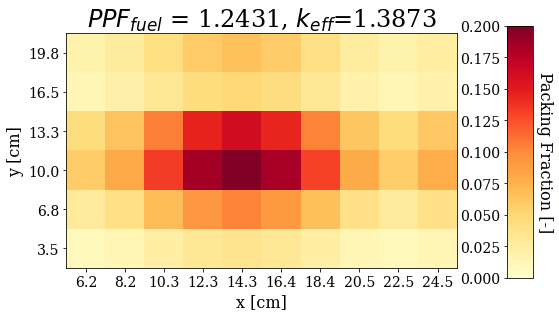
\includegraphics[width=0.49\linewidth]{a-1c-ppf-triso-comparison-least-minimized.png} 
    \caption{Simulation a-1c's most-minimized $PPF_{fuel}$ TRISO distribution 
    from Figure \ref{fig:assem-obj-1-ppf} (left) and the highest $PPF_{fuel}$ TRISO 
    distribution (right).}
    \label{fig:a-1c-ppf-triso-comparison}
\end{figure}

Figure \ref{fig:a-1c-flux-comparison} compares the 4 energy group flux distributions 
between simulation a-1c's most-minimized $PPF_{fuel}$ TRISO distribution and highest 
$PPF_{fuel}$ TRISO distribution (both shown in Figure \ref{fig:a-1c-ppf-triso-comparison}). 
\begin{figure}[htbp!]
    \centering
    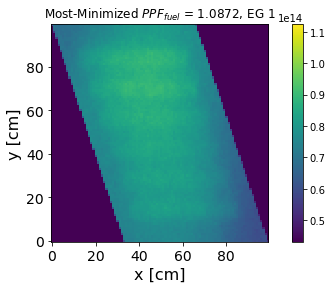
\includegraphics[width=0.35\linewidth]{flux-comparison-a-1c-most-minimized-grp1.png} 
    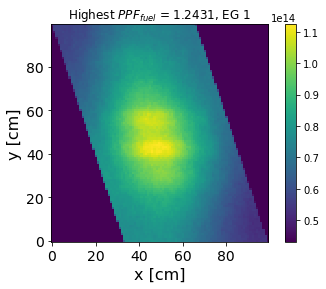
\includegraphics[width=0.35\linewidth]{flux-comparison-a-1c-least-minimized-grp1.png} 
    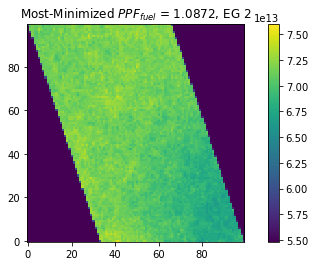
\includegraphics[width=0.35\linewidth]{flux-comparison-a-1c-most-minimized-grp2.png} 
    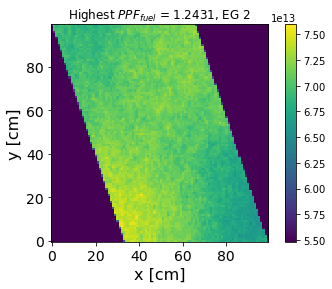
\includegraphics[width=0.35\linewidth]{flux-comparison-a-1c-least-minimized-grp2.png} 
    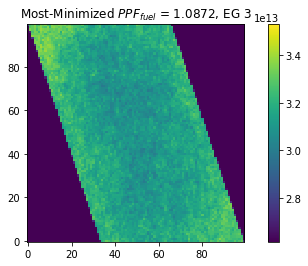
\includegraphics[width=0.35\linewidth]{flux-comparison-a-1c-most-minimized-grp3.png} 
    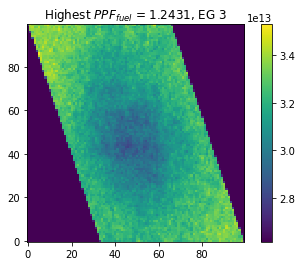
\includegraphics[width=0.35\linewidth]{flux-comparison-a-1c-least-minimized-grp3.png} 
    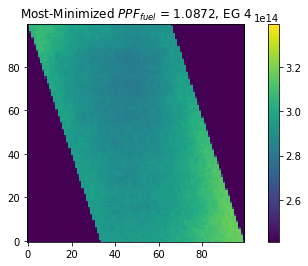
\includegraphics[width=0.35\linewidth]{flux-comparison-a-1c-most-minimized-grp4.png} 
    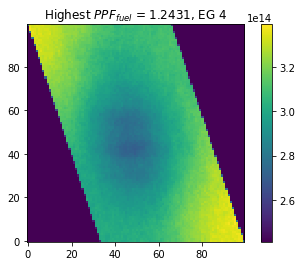
\includegraphics[width=0.35\linewidth]{flux-comparison-a-1c-least-minimized-grp4.png} 
    \caption{AHTR one-third assembly's flux comparison between the two reactor models 
    in Figure \ref{fig:a-1c-ppf-triso-comparison}: simulation a-1c's most-minimized 
    $PPF_{fuel}$ reactor model with $PPF_{fuel} = 1.0872$ and simulation a-1c's reactor 
    model with the highest $PPF_{fuel} = 1.2431$.
    Energy Group 1: E $> 9.1188 \times 10^{-3}$ MeV, 
    Energy Group 2: $2.9023 \times 10^{-5} < E < 9.1188 \times 10^{-3}$ MeV,
    Energy Group 3:  $1.8556 \times 10^{-5} < E < 2.9023 \times 10^{-5}$ MeV,
    Energy Group 4:  $1.0 \times 10^{-12} < E < 1.8554 \times 10^{-6}$ MeV.}
    \label{fig:a-1c-flux-comparison}
\end{figure}
In Figure \ref{fig:a-1c-flux-comparison}, the reactor model with the highest 
$PPF_{fuel} = 1.2431$'s Group 4 flux dips in the center of the one-third assembly 
due to spatial self-shielding effects. 
In the highest $PPF_{fuel} = 1.2431$ reactor model's Group 1 flux, there is a peak in 
fast neutrons born in the one-third assembly's center, the fast neutrons are moderated 
in the graphite matrix and graphite structure (\gls{AHTR} one-third assembly 
geometry: Figure \ref{fig:ahtr_assembly}). 
The moderated neutrons are more likely absorbed at the fuel regions nearer to 
the outer pure graphite structure moderating regions. 

Table \ref{tab:a-1c-flux-comparison} quantifies the total flux differences per energy 
group between the compared reactor models. 
The flux values were tallied for each energy group within the one-third assembly model 
using a 100 x 100 mesh. 
\begin{table}[htbp!]
    \centering
    \onehalfspacing
    \caption{Flux value comparison between the two reactor models in Figure 
    \ref{fig:a-1c-ppf-triso-comparison}: simulation a-1c's most-minimized $PPF_{fuel}$ reactor model 
    with $PPF_{fuel} = 1.0872$ and simulation a-1c's reactor model with the highest 
    $PPF_{fuel} = 1.2431$.
    Energy Group 1: E $> 9.1188 \times 10^{-3}$ MeV, 
    Energy Group 2: $2.9023 \times 10^{-5} < E < 9.1188 \times 10^{-3}$ MeV,
    Energy Group 3:  $1.8556 \times 10^{-5} < E < 2.9023 \times 10^{-5}$ MeV,
    Energy Group 4:  $1.0 \times 10^{-12} < E < 1.8554 \times 10^{-6}$ MeV.}
	\label{tab:a-1c-flux-comparison}
    \footnotesize
    \begin{tabular}{lp{4cm}p{4cm}p{3cm}}
    \hline
    \textbf{Energy Group} &
    \textbf{$max(\phi)/min(\phi)$ Most-minimized $PPF_{fuel}$ TRISO Distribution} & 
    \textbf{$max(\phi)/min(\phi)$ Highest $PPF_{fuel}$ TRISO Distribution} & 
    \textbf{$\%$ Difference}\\
    \hline 
    1 & 1.825 & 2.608 & \Minus30.00 \\
    2 & 1.341 & 1.386 & \Minus3.18 \\
    3 & 1.302 & 1.334 & \Minus2.43 \\
    4 & 1.319 & 1.331 & \Minus0.85 \\
    \hline
    \end{tabular}
\end{table}

In energy group 4, the most-minimized $PPF_{fuel}$ flux distribution is $0.85\%$ flatter 
than the reactor model with the highest $PPF_{fuel} = 1.2431$.
These results verify that similar to the \gls{AHTR} plank model, the \gls{AHTR} one-third 
assembly model's minimize $PPF_{fuel}$ objective is also driven by flattening thermal 
(Group 4) flux distribution since $max(\Phi_j) \div ave(\Phi_j) \propto PPF_{fuel}$
(Equation \ref{eq:flux-prop-ppf}). 

\paragraph{Simulation p-1f}
In Section \ref{sec:assem-1-obj-ppf}'s simulation a-1f, I conducted a single-objective 
optimization simulation to minimize fuel-normalized power peaking factor ($PPF_{fuel}$) by 
varying coolant channel shape. 
In simulation a-1f, \gls{ROLLO} found that there is no correlation 
between $PPF_{fuel}$ and coolant channel shape (demonstrated in Figure 
\ref{fig:a-1f}). 

\paragraph{Summary}
I verified that the minimize $PPF_{fuel}$ objective for the \gls{AHTR} one-third assembly 
model is also driven by flattening thermal (Group 4) flux distribution. 
The minimize $PPF_{fuel}$ objective influences $PF_{total}$ and oscillations in the 
TRISO disribution.
The objective has no correlation with coolant channel shape input parameter.

\subsection{Discussion: Multi-Objective Optimization}
\label{sec:assem-discussion-multi}
\gls{ROLLO} successfully found widely spread out reactor model solutions in each of the 
multi-objective optimization simulation's final generation Pareto fronts.
In this section, I explain how the driving factors and phenomena observed in 
the previous single-objective discussions (Sections 
\ref{sec:assem-discussion-pf}, \ref{sec:assem-discussion-temp}, and 
\ref{sec:assem-discussion-ppf}) combine to result in the optimal reactor models found 
by the multi-objective optimization simulations. 

\subsubsection{Simulation a-2a}
In Section \ref{sec:a-2a}'s simulation a-2a, I conducted a two-objective 
optimization simulation to minimize total fuel packing fraction ($PF_{total}$) and 
maximum temperature ($T_{max}$) in a one-third assembly model by varying $PF_{total}$ 
and TRISO distribution. 
In simulation a-2a, ROLLO found 13 reactor models on the Pareto Front (Figure 
\ref{fig:assem-obj-2-pftemp-pareto}). 

In simulation a-2a, \gls{ROLLO} found that the one-third assembly models with the 
most-minimized $PF_{total}$ objective are reactor models 3 and 4 (Figure 
\ref{fig:assem-obj-2-pftemp-pareto-distr}). 
Both reactor models have an oscillating TRISO distribution along the both the x-axis 
and y-axis. 
Figure \ref{fig:a-2a-pf-triso-comparison} compares simulation a-2a's most-minimized 
$PF_{total}$ reactor model 3 and simulation a-1a's most-minimized $PF_{total}$ reactor 
model. 
\begin{figure}[htbp!]
    \centering
    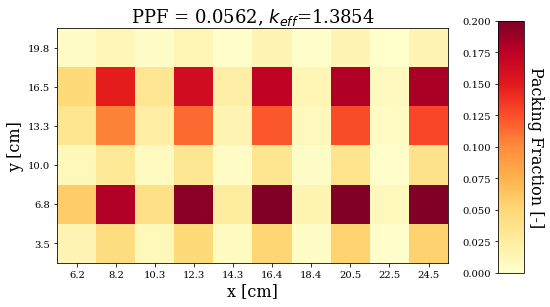
\includegraphics[width=0.49\linewidth]{a-2a-pf-most-minimized.png} 
    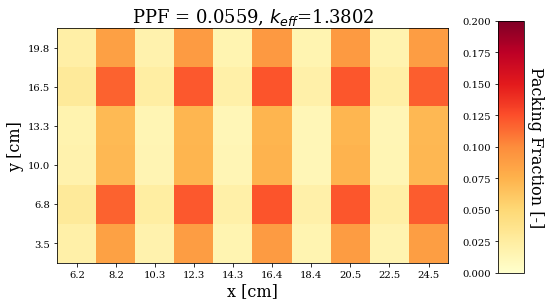
\includegraphics[width=0.49\linewidth]{assem-0.0559-most-minimized.png} 
    \caption{Simulation a-2a's most-minimized $PF_{total}$ TRISO distribution 
    from Figure \ref{fig:assem-obj-2-pftemp} (left) and simulation a-1a's 
    most-minimized $PF_{total}$ TRISO distribution from Figure 
    \ref{fig:assem-obj-1-pf} (right).}
    \label{fig:a-2a-pf-triso-comparison}
\end{figure}
Figure \ref{fig:a-2a-pf-triso-comparison} shows that simulation a-2a's most-minimized 
$PF_{total}$ reactor model and simulation a-1a's most-minimized $PF_{total}$ reactor 
model have similar distributions with peaks on the even fuel cell columns, but at 
different amplitudes. 

In simulation a-2a, \gls{ROLLO} found that the one-third assembly model with the 
most-minimized $T_{max}$ objective, reactor model 9 (Figure 
\ref{fig:assem-obj-2-pftemp-pareto-distr}), has an almost constant TRISO distribution.
Figure \ref{fig:a-2a-temp-triso-comparison} compares simulation a-2a's most-minimized 
$T_{max}$ reactor model 9 and simulation a-1b's most-minimized $T_{max}$ reactor model. 
\begin{figure}[htbp!]
    \centering
    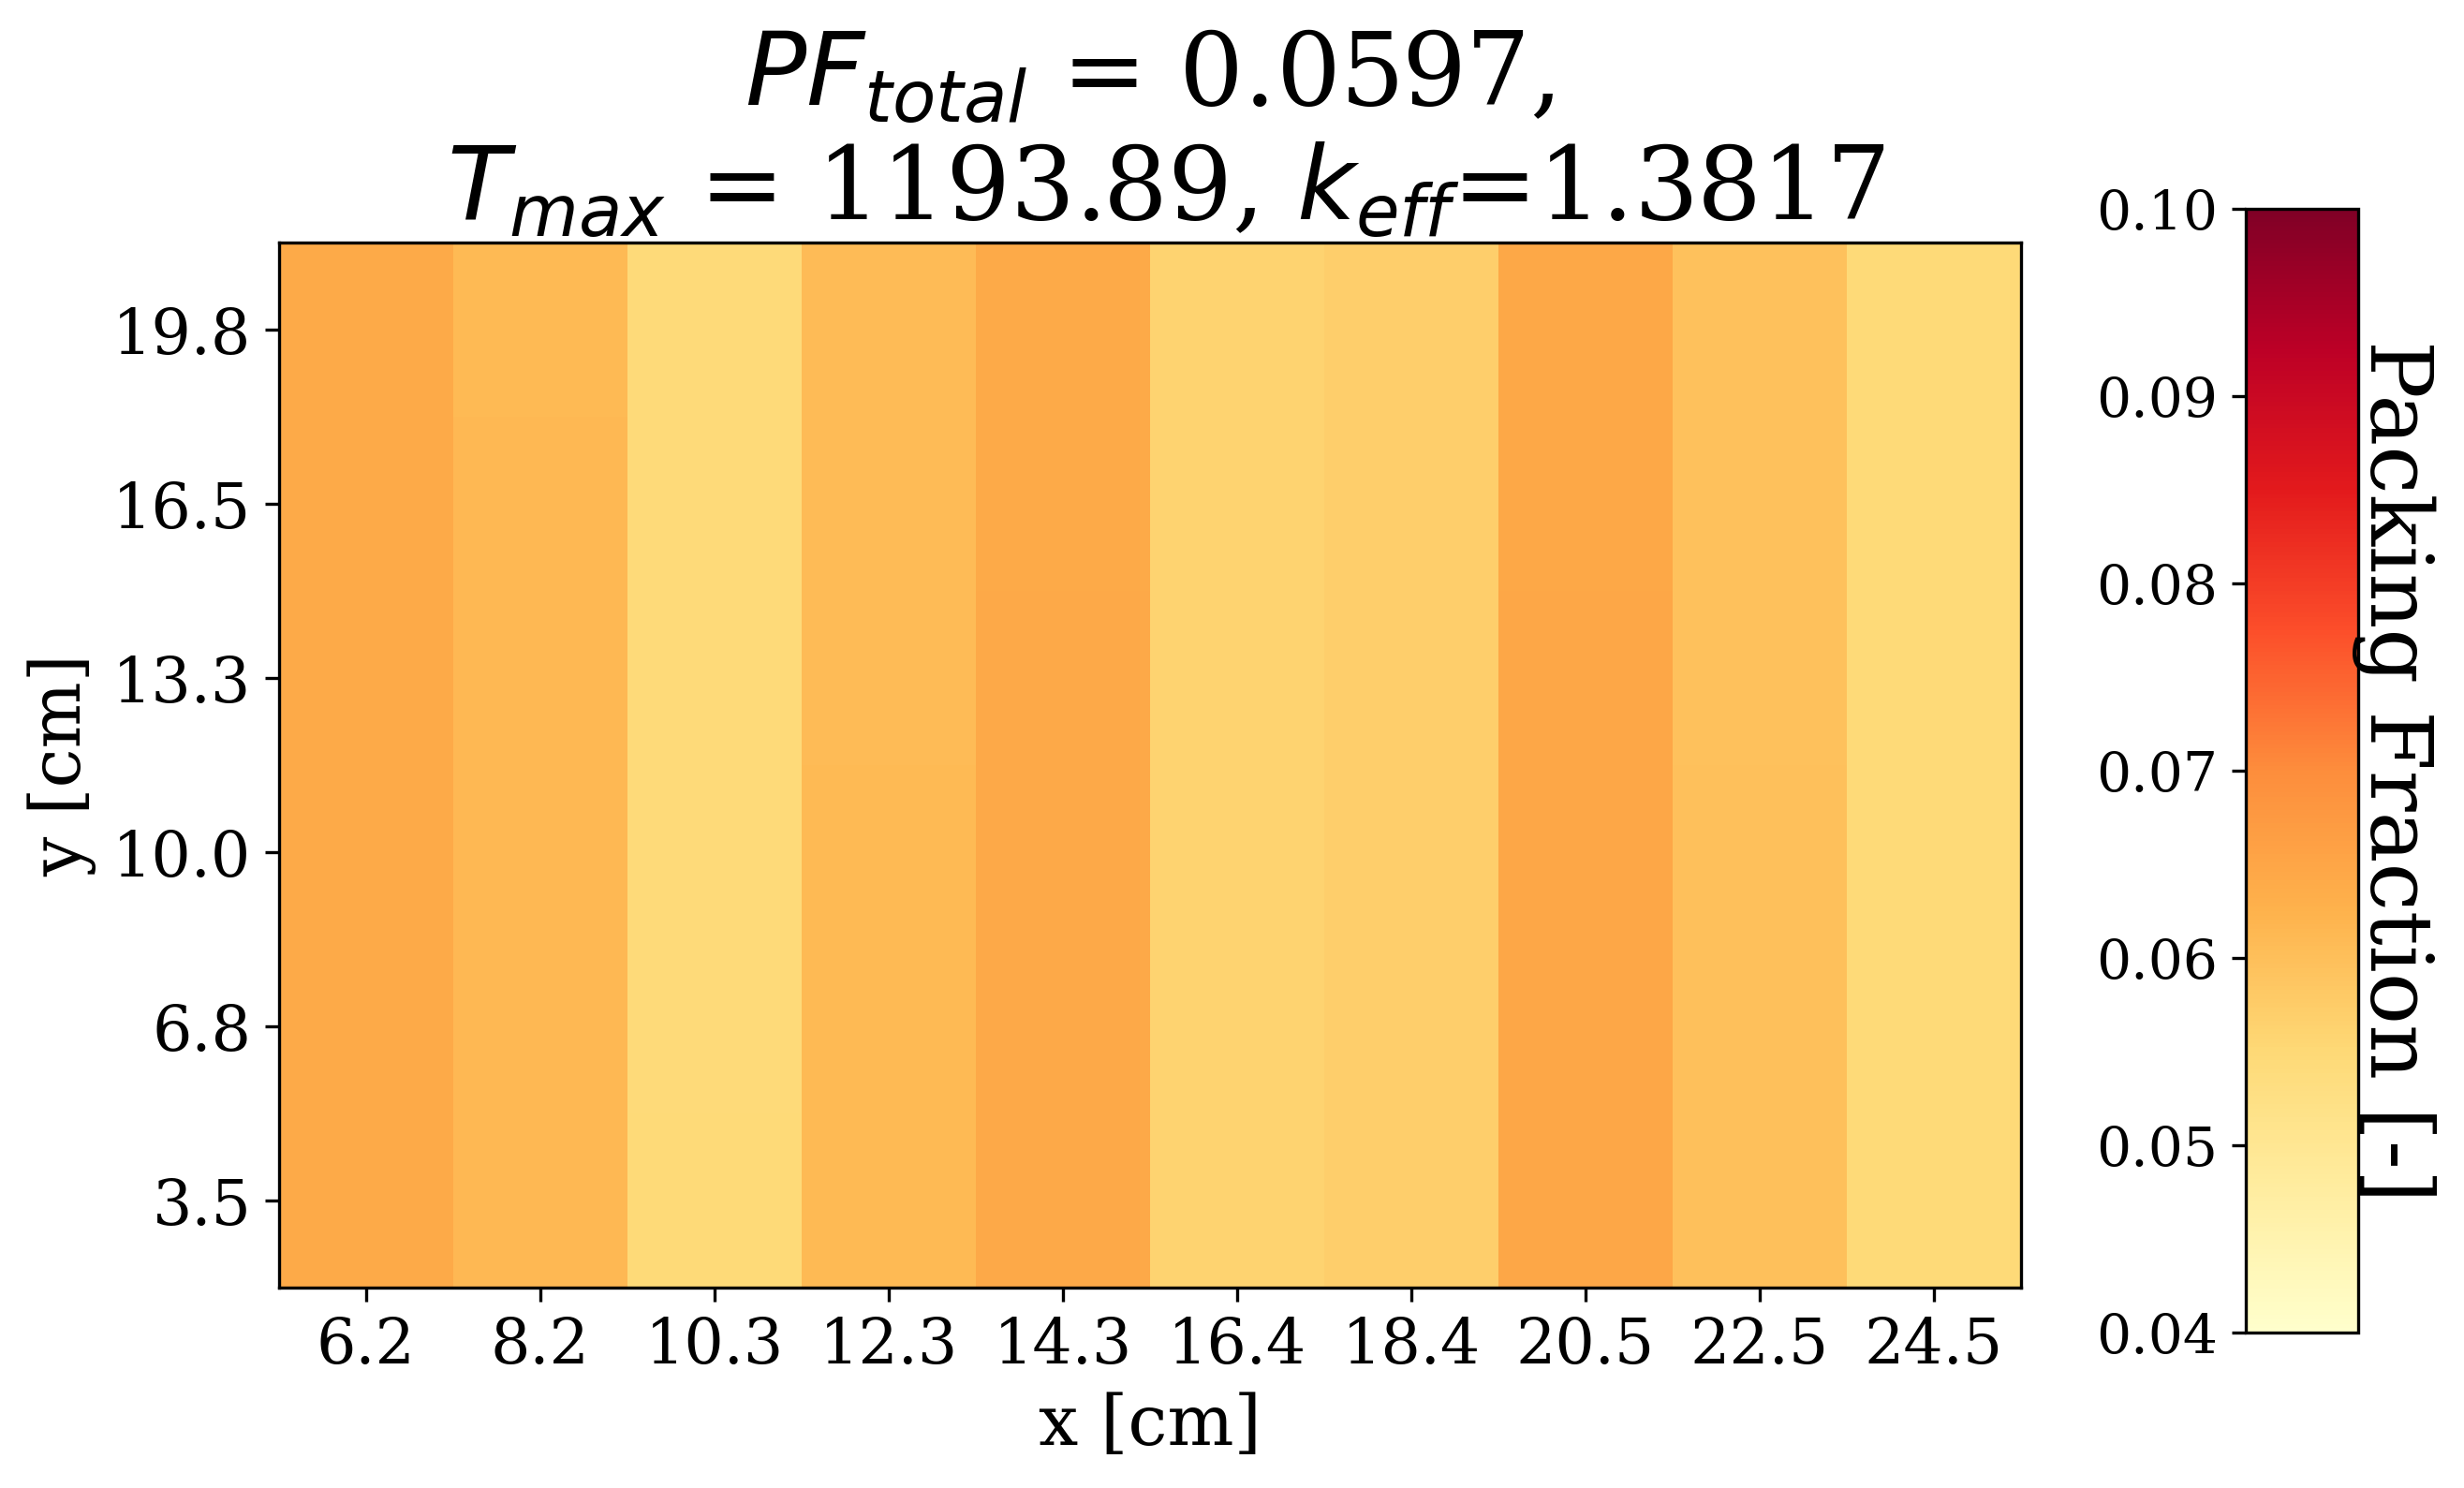
\includegraphics[width=0.49\linewidth]{a-2a-temp-most-minimized.png} 
    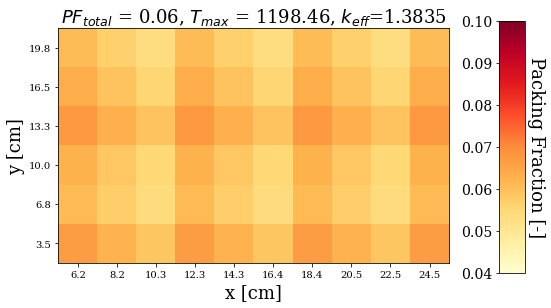
\includegraphics[width=0.49\linewidth]{a-1b-temp-most-minimized.png} 
    \caption{Simulation a-2a's most-minimized $T_{max}$ TRISO distribution 
    from Figure \ref{fig:assem-obj-2-pftemp} (left) and simulation a-1b's 
    most-minimized $T_{max}$ TRISO distribution from Figure 
    \ref{fig:assem-obj-1-temp} (right).}
    \label{fig:a-2a-temp-triso-comparison}
\end{figure}
Figure \ref{fig:a-2a-temp-triso-comparison} shows that simulation a-2a's most-minimized 
$T_{max}$ reactor model and simulation a-1b's most-minimized $T_{max}$ reactor model 
have similar almost constant TRISO distributions with packing fraction standard 
deviations of $0.004$ and $0.0009$, respectively.
However, they have different $PF_{total}$ values, and simulation a-2a's most-minimized 
$T_{max}$'s TRISO distribution is not as flat as simulation a-1b. 

Figure \ref{fig:a-2a-balanced-reactor-model} shows reactor model 13 which 
minimized both $PF_{total}$ and $T_{max}$ to an equal extent by balancing influences 
from both objectives. 
\begin{figure}[htbp!]
    \centering
    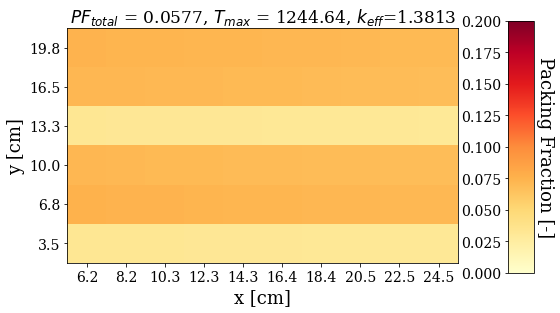
\includegraphics[width=0.6\linewidth]{a-2a-balanced-reactor-model.png} 
    \caption{Simulation a-2a's reactor model 13 which minimized both $PF_{total}$ and $T_{max}$ 
    to an equal extent (see Pareto Front in Figure \ref{fig:assem-obj-2-pftemp}).}
    \label{fig:a-2a-balanced-reactor-model}
\end{figure}
The \gls{TRISO} distributions on simulation a-2a's Pareto front in Figure 
\ref{fig:assem-obj-2-pftemp} minimize both $PF_{total}$ and $T_{max}$, and vary
between the two extreme cases: most-minimized $PF_{total}$ and most-minimized $T_{max}$. 
The minimize $T_{max}$ objective influences the TRISO distribution's flatness as 
described in Section \ref{sec:assem-discussion-temp}, while 
the minimize $PF_{total}$ objective influences the oscillating pattern, as described 
in Section \ref{sec:assem-discussion-pf}.

\subsubsection{Simulation a-2b}
% compare reactor models 1,3,5's fission reaction rate and thermal flux flattness
In Section \ref{sec:a-2b}'s simulation a-2b, I conducted a two-objective 
optimization simulation to minimize total fuel packing fraction ($PF_{total}$) and 
fuel-normalized power peaking factor ($PPF_{fuel}$) in a one-third assembly model 
by varying $PF_{total}$ and TRISO packing fraction distribution. 
In simulation a-2b's final generation, ROLLO found 12 reactor models on the Pareto Front 
(Figure \ref{fig:assem-obj-2-pfppf-pareto}). 

In simulation a-2b, \gls{ROLLO} found that the one-third assembly model with the 
most-minimized $PF_{total}$ objective, reactor model 3 (Figure 
\ref{fig:assem-obj-2-pfppf-pareto-distr}), has an oscillating TRISO distribution 
along the both the x-axis and y-axis. 
Figure \ref{fig:a-2b-pf-triso-comparison} compares simulation a-2b's reactor model 3 and 
simulation a-1a's most-minimized $PF_{total}$ reactor model. 
\begin{figure}[htbp!]
    \centering
    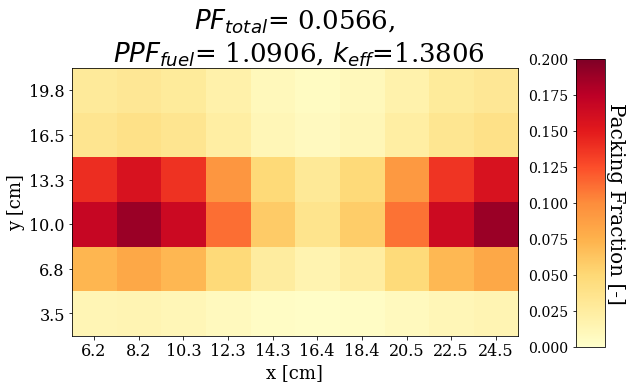
\includegraphics[width=0.49\linewidth]{a-2b-pf-most-minimized.png} 
    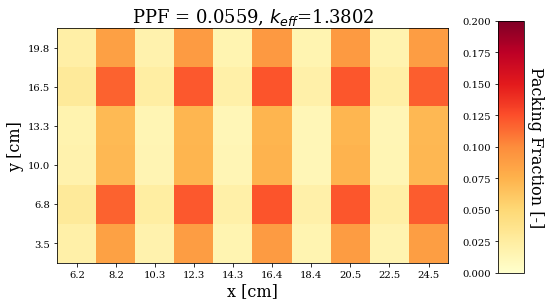
\includegraphics[width=0.49\linewidth]{assem-0.0559-most-minimized.png} 
    \caption{Simulation a-2b's most-minimized $PF_{total}$ TRISO distribution 
    from Figure \ref{fig:assem-obj-2-pfppf} (left) and simulation a-1a's 
    most-minimized $PF_{total}$ TRISO distribution from Figure 
    \ref{fig:assem-obj-1-pf} (right).}
    \label{fig:a-2b-pf-triso-comparison}
\end{figure}
Figure \ref{fig:a-2b-pf-triso-comparison} shows that simulation a-2b's reactor model 3 
and simulation a-1a's most-minimized $PF_{total}$ reactor model have similarly large 
packing fraction standard deviation of $0.053$ and $0.04$, respectively. 
However, they do not follow the same TRISO distribution pattern. 
Section \ref{sec:plank-discussion-ppf} described that in the \gls{AHTR} plank model, 
the minimize $PF_{total}$ and minimize $PPF_{fuel}$ objectives influence each other
resulting in unexpected TRISO distributions at different $PF_{total}$ values.
This same effect also applies to the one-third assembly model, explaining why unlike 
simulation a-2a, simulation a-2b's extreme most-minimized $PF_{total}$ and 
most-minimized $PPF_{fuel}$ do not follow similar TRISO distribution patterns as their 
single-objective counterparts.

In simulation a-2b, \gls{ROLLO} found that the one-third assembly model with the 
most-minimized $PPF_{fuel}$ objective, reactor model 1 (Figure 
\ref{fig:assem-obj-2-pfppf-pareto-distr}) has a TRISO distribution that oscillates
along the y-axis and oscillates slightly along the x-axis. 
Figure \ref{fig:a-2b-pf-triso-comparison} compares simulation a-2b's most-minimized 
$PPF_{fuel}$ reactor model 1 and simulation a-1c's most-minimized $PPF_{fuel}$ reactor 
model. 
\begin{figure}[htbp!]
    \centering
    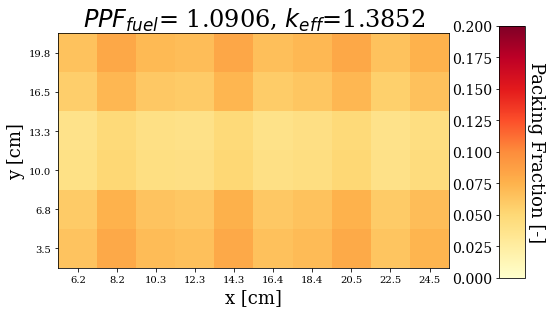
\includegraphics[width=0.49\linewidth]{a-2b-ppf-most-minimized.png} 
    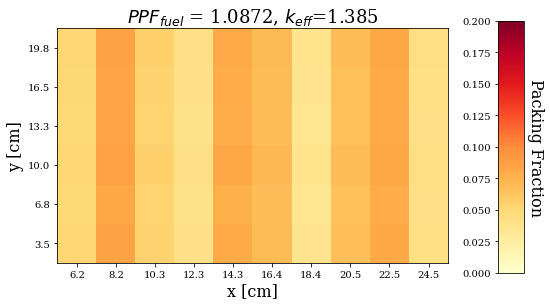
\includegraphics[width=0.49\linewidth]{a-1c-ppf-triso-comparison-most-minimized.png} 
    \caption{Simulation a-2b's most-minimized $PPF_{fuel}$ TRISO distribution 
    from Figure \ref{fig:assem-obj-2-pfppf} (left) and simulation a-1c's 
    most-minimized $PPF_{fuel}$ TRISO distribution from Figure 
    \ref{fig:assem-obj-1-ppf} (right).}
    \label{fig:a-2b-ppf-triso-comparison}
\end{figure}
Figure \ref{fig:a-2b-ppf-triso-comparison} shows that simulation a-2b's reactor model 1 
and simulation a-1a's most-minimized $PPF_{fuel}$ reactor model have similarly small 
packing fraction standard deviation of $0.013$ and $0.017$, respectively. 
However, they do not follow the same TRISO distribution pattern, this is
attributed to the $PF_{total}$ and $PPF_{fuel}$ relationship resulting in unexpected 
TRISO distributions at different $PF_{total}$ values, as mentioned previously. 
The relationship between the \gls{AHTR}'s $PF_{total}$ and $PPF_{fuel}$ 
merits future work of further sensitivity analysis. 

To better understand the reactor models on simulation a-2b's Pareto Front, I do a 
deep dive into the driving factors for the minimize $PF_{total}$ and minimize 
$PPF_{fuel}$ objectives. 

\paragraph{Driving Factor Quantification}
Sections \ref{sec:assem-discussion-pf} and \ref{sec:assem-discussion-ppf} 
verified that similar to the \gls{AHTR} plank, the \gls{AHTR} one-third assembly's 
minimize $PF_{total}$ objective is driven by maximizing total fission reaction 
rates, and the minimize $PPF_{fuel}$ objective is driven by flattening the thermal flux 
distribution. 
This section compares the total fission reaction rate and thermal flux flatness for 
3 reactors models on simulation a-2b's Pareto Front (Figure 
\ref{fig:assem-obj-2-pfppf-pareto}): reactor model 11 with most-minimized $PF_{total}$, 
reactor model 1 with most-minimized $PPF_{fuel}$, and reactor model 5 that minimizes 
both $PF_{total}$ and $PPF_{fuel}$ to an equal extent.
Figure \ref{fig:a-2b-comparison-reactors} shows the TRISO packing fraction distribution 
for the 3 reactors models.
\begin{figure}[htbp!]
    \centering
    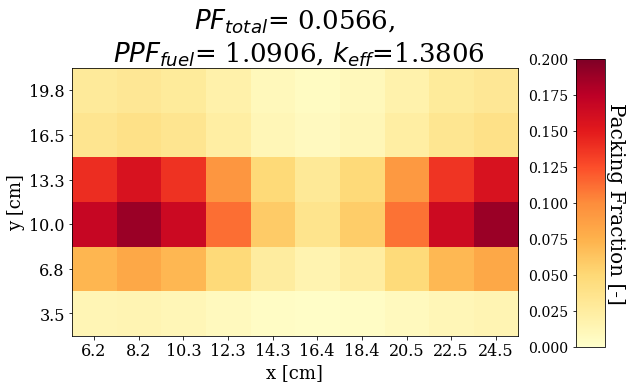
\includegraphics[width=0.49\linewidth]{a-2b-pf-most-minimized.png} 
    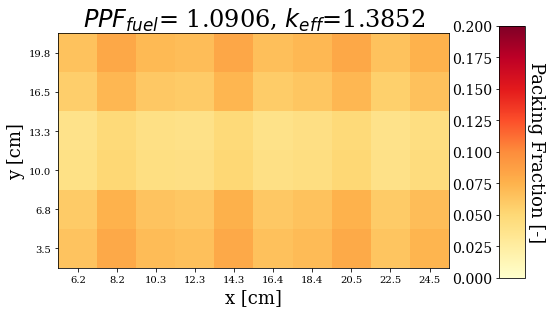
\includegraphics[width=0.49\linewidth]{a-2b-ppf-most-minimized.png} 
    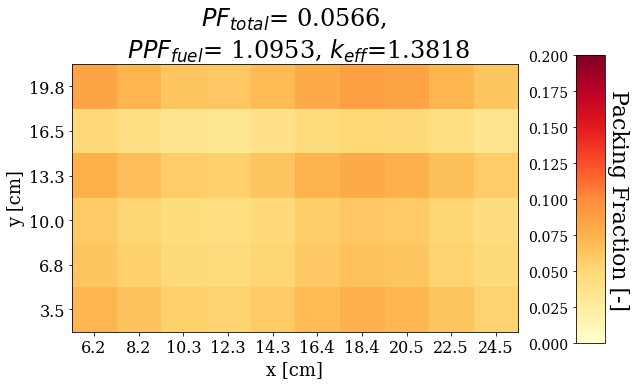
\includegraphics[width=0.49\linewidth]{a-2b-both-most-minimized.png} 
    \caption{TRISO distributions for 3 reactor models on Simulation a-2b's Pareto Front 
    (Figure \ref{fig:assem-obj-2-pfppf-pareto}): reactor model 11 with most-minimized 
    $PF_{total}$ (top left), reactor model 1 with most-minimized $PPF_{fuel}$ (top right), 
    and reactor model 5 that minimizes both $PF_{total}$ and $PPF_{fuel}$ to an equal 
    extent (bottom).}
    \label{fig:a-2b-comparison-reactors}
\end{figure}

Table \ref{tab:a-2b-comparison-reactors} shows the total fission reaction rate, 
and thermal flux flatness for the three reactor models. 
\begin{table}[htbp!]
    \centering
    \onehalfspacing
    \caption{
    Total fission reaction rate, and thermal flux flatness ($max(\phi_4)/min(\phi_4)$) 
    for 3 reactor models on simulation a-2b's Pareto Front (Figure 
    \ref{fig:assem-obj-2-pfppf-pareto}): reactor model 1 with most-minimized 
    $PPF_{fuel}$, reactor model 11 with most-minimized $PF_{total}$, and reactor model 
    5 that minimizes both $PF_{total}$ and $PPF_{fuel}$ to an equal extent.}
	\label{tab:a-2b-comparison-reactors}
    \footnotesize
    \begin{tabular}{p{3cm}p{1.5cm}p{2.3cm}lp{2.5cm}l}
    \hline
    \textbf{Most Minimized Parameter} & \textbf{Reactor Model} 
    & \textbf{Fission \newline [reactions/src]} & \textbf{$\%$ Diff}
    & $max(\phi_4)/min(\phi_4)$ & \textbf{$\%$ Diff}\\
    \hline 
    Both & 5 & 0.5471 & - & 1.2986 & -\\
    \textbf{$PF_{total}$} & 11 & 0.5472 & \Plus0.017 & 1.3168 & \Plus1.40\\
    \textbf{$PPF_{fuel}$} & 1 & 0.5478 & \Plus0.12 & 1.2851 & \Minus1.03\\
    \hline
    \end{tabular}
\end{table}

The most minimized $PPF_{fuel}$ reactor model 1 has the highest fission reaction rate, 
followed by the most minimized $PF_{total}$ reactor model 11, and then reactor model 5 
that minimizes both $PF_{total}$ and $PPF_{fuel}$ to an equal extent.
Reactor model 1 has the highest fisson reaction rate since it has the highest 
$PF_{total}$.
Reactor model 11 has a slightly higher fission reaction rate compared to reactor model 5 
and they have $k_{eff}$ values within error of each other despite reactor model 11 
having a lower $PF_{total}$ ($PF_{total, 11}=0.0566$ vs. $PF_{total, 5}=0.0591$).
Section \ref{sec:assem-discussion-pf} verified that the \gls{AHTR} one-third assembly 
model's minimize $PF_{total}$ objective is driven by maximizing total fission reaction 
rate.
Therefore, reactor model 11's oscillating TRISO distribution enables a lower 
$PF_{total}$ for the same $k_{eff}$ as reactor model 5 since both reactor models 
have comparable total fission reaction rates. 

The most minimized $PPF_{fuel}$ reactor model 1 has the flattest thermal flux, followed by 
reactor model 5 that minimizes both $PF_{total}$ and $PPF_{fuel}$ to an equal extent, and 
then the most minimized $PF_{fuel}$ reactor model 11. 
Section \ref{sec:assem-discussion-ppf} verified that the \gls{AHTR} one-third assembly 
model's minimize $PPF_{fuel}$ objective is driven by flattening thermal (Group 4) flux 
distribution. 
Therefore, reactor model 1 with the flattest thermal flux distribution most minimized 
$PPF_{fuel}$. 

\subsubsection{Simulation a-2c}
In Section \ref{sec:a-2c}'s simulation a-2c, I conducted a two-objective 
optimization simulation to minimize maximum temperature ($T_{max}$) and fuel-normalized 
power peaking factor ($PPF_{fuel}$) in a one-third assembly model by varying 
TRISO distribution. 
In simulation a-2c, ROLLO found 1 reactor model on the Pareto Front (Figure 
\ref{fig:assem-obj-2-tempppf-pareto}), demonstrating that minimize $T_{max}$ and 
minimize $PPF_{fuel}$ objectives are non-contrasting for the one-third assembly model. 

Figure \ref{fig:a-2c-triso-comparison} compares the single reactor model on simulation 
a-2c's Pareto Front, simulation a-1b's most-minimized $T_{max}$ reactor model, and 
simulation a-1c's most-minimized $PPF_{fuel}$ reactor model. 
All reactor models have $PF_{total}=0.06$.
\begin{figure}[htbp!]
    \centering
    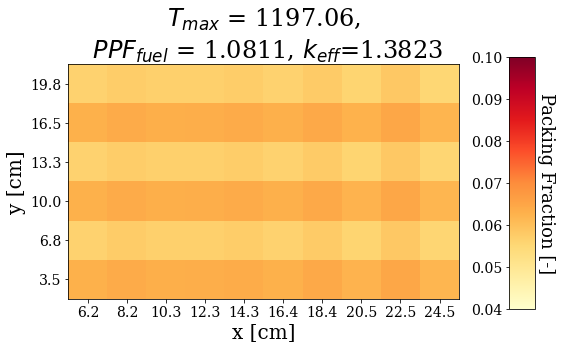
\includegraphics[width=0.51\linewidth]{a-2c-most-minimized.png} 
    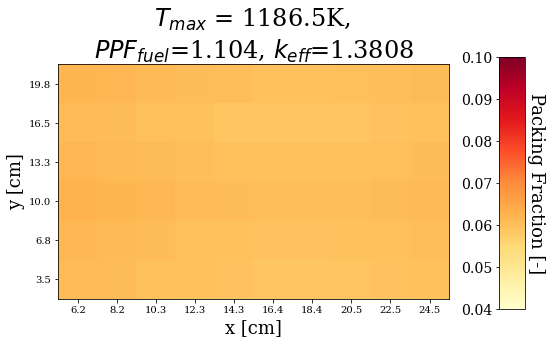
\includegraphics[width=0.49\linewidth]{a-1b-temp-most-minimized-with-ppf.png} 
    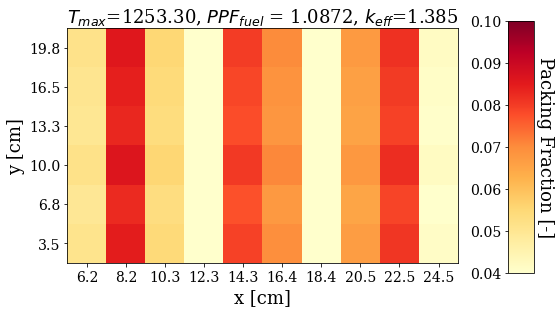
\includegraphics[width=0.49\linewidth]{a-1c-ppf-triso-comparison-most-minimized-01-scale.png} 
    \caption{Simulation a-2c's single Pareto Front reactor model's TRISO distribution 
    from Figure \ref{fig:assem-obj-2-tempppf} (above), simulation a-1b's most-minimized 
    $T_{max}$ TRISO distribution from Figure \ref{fig:assem-obj-1-temp} (lower left), and 
    simulation a-1c's most-minimized $PPF_{fuel}$ TRISO distribution from Figure 
    \ref{fig:assem-obj-1-ppf} (lower right).
    All reactor models have $PF_{total}=0.06$.}
    \label{fig:a-2c-triso-comparison}
\end{figure}

Figure \ref{fig:a-2c-triso-comparison} shows that the single reactor model on simulation 
a-2c's Pareto Front's TRISO distributions is more similar to simulation a-1b's 
most-minimized $T_{max}$ TRISO distribution than simulation a-1c's most-minimized 
$PPF_{fuel}$ TRISO distribution. 
Simulation a-1c's most-minimized $PPF_{fuel}$ reactor model has a high $T_{max}=1253.30$ 
K, while simulation a-1b's most-minimized $T_{max}$ reactor model has a low 
$PPF_{fuel}=1.104$. 
Therefore, influences from the minimize $T_{max}$ objective, results in the single 
reactor model on simulation a-2c's Pareto Front to have a TRISO distribution more 
similar to simulation a-1b's most-minimized $T_{max}$ reactor model. 
The minimize $T_{max}$ objective influences the TRISO distribution's flatness as 
described in Section \ref{sec:assem-discussion-temp}, while 
the minimize $PPF_{fuel}$ objective influences the oscillating pattern, as described 
in Section \ref{sec:assem-discussion-ppf}.

\subsubsection{Simulation a-3a}
In Section \ref{sec:a-3a}'s simulation a-3a, I conducted a three-objective 
optimization simulation to minimize total fuel packing fraction ($PF_{total}$), 
maximum temperature ($T_{max}$), and fuel-normalized power peaking factor 
($PPF_{fuel}$) in the one-third assembly model by varying $PF_{total}$ and 
TRISO distribution.
\gls{ROLLO} found 32 widely spread reactor models on simulation a-3a's Pareto 
front (Figure \ref{fig:assem-obj-3-2d}). 

In simulation a-3a, \gls{ROLLO} found that the one-third assembly model with the 
most-minimized $PF_{total}$ objective, reactor model 30 (Figure 
\ref{fig:assem-obj-3-most-minimized-distr}), has an oscillating TRISO distribution 
along the both the x-axis and y-axis. 
Figure \ref{fig:a-3a-pf-triso-comparison} compares simulation a-3a's reactor model 30 and 
simulation a-1a's most-minimized $PF_{total}$ reactor model. 
\begin{figure}[htbp!]
    \centering
    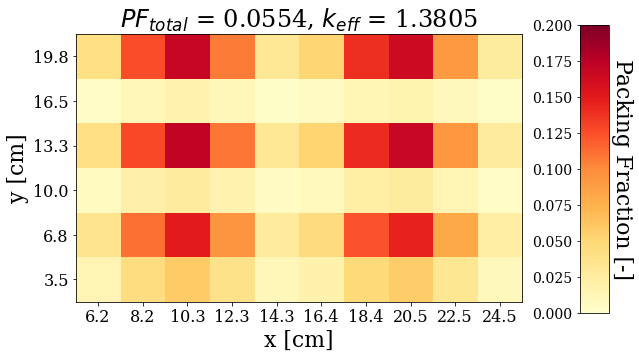
\includegraphics[width=0.49\linewidth]{a-3a-pf-most-minimized.png} 
    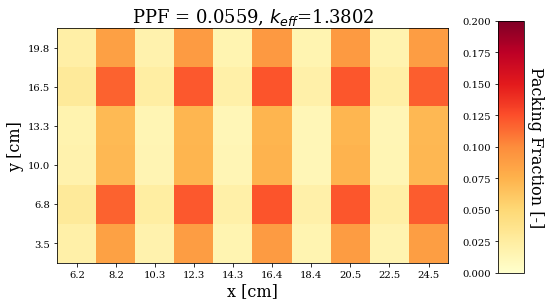
\includegraphics[width=0.49\linewidth]{assem-0.0559-most-minimized.png} 
    \caption{Simulation a-3a's most-minimized $PF_{total}$ TRISO distribution 
    from Figure \ref{fig:assem-obj-3-most-minimized} (left) and simulation a-1a's 
    most-minimized $PF_{total}$ TRISO distribution from Figure 
    \ref{fig:assem-obj-1-pf} (right).}
    \label{fig:a-3a-pf-triso-comparison}
\end{figure}
Figure \ref{fig:a-3a-pf-triso-comparison} shows that simulation a-3a's reactor model 30 
and simulation a-1a's most-minimized $PF_{total}$ reactor model have similarly large 
packing fraction standard deviation of $0.052$ and $0.04$, respectively. 
However, they do not follow the same TRISO distribution pattern, this could be 
attributed to the $PF_{total}$ and $PPF_{fuel}$ relationship resulting in unexpected 
TRISO distributions at different $PF_{total}$ values, as mentioned previously. 

In simulation a-3a, \gls{ROLLO} found that the one-third assembly model with the 
most-minimized $T_{max}$ objective, reactor model 3 (Figure 
\ref{fig:assem-obj-3-most-minimized-distr}), has an almost constant TRISO distribution.
Figure \ref{fig:a-3a-temp-triso-comparison} compares simulation a-3a's most-minimized 
$T_{max}$ reactor model 3 and simulation a-1b's most-minimized $T_{max}$ reactor model. 
\begin{figure}[htbp!]
    \centering
    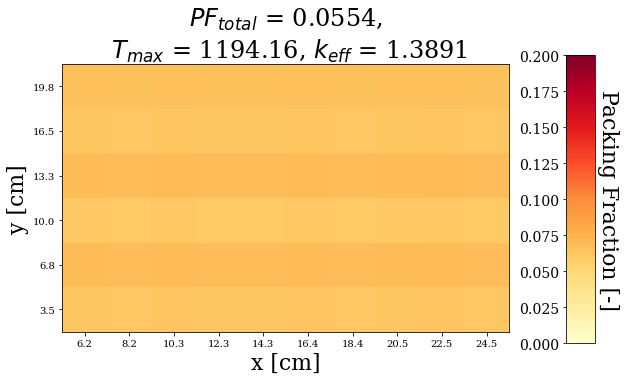
\includegraphics[width=0.49\linewidth]{a-3a-temp-most-minimized.png} 
    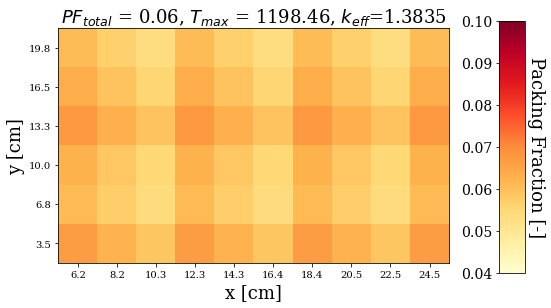
\includegraphics[width=0.49\linewidth]{a-1b-temp-most-minimized.png} 
    \caption{Simulation a-3a's most-minimized $T_{max}$ TRISO distribution 
    from Figure \ref{fig:assem-obj-3-most-minimized-distr} (left) and simulation a-1b's 
    most-minimized $T_{max}$ TRISO distribution from Figure 
    \ref{fig:assem-obj-1-temp} (right).}
    \label{fig:a-3a-temp-triso-comparison}
\end{figure}
Figure \ref{fig:a-3a-temp-triso-comparison} shows that simulation a-3a's most-minimized 
$T_{max}$ reactor model and simulation a-1b's most-minimized $T_{max}$ reactor model 
have similar almost constant TRISO distributions with packing fraction standard 
deviations of $0.003$ and $0.0009$, respectively.
However, they have different $PF_{total}$ values, and simulation a-3a's most-minimized 
$T_{max}$'s TRISO distribution is not as flat as simulation a-1b. 

In simulation a-3a, \gls{ROLLO} found that the one-third assembly model with the 
most-minimized $PPF_{fuel}$ objective, reactor model 1 (Figure 
\ref{fig:assem-obj-3-most-minimized-distr}) has an oscillating TRISO distribution 
along the both the x-axis and y-axis.
Figure \ref{fig:a-3a-ppf-triso-comparison} compares simulation a-3a's most-minimized 
$PPF_{fuel}$ reactor model 1 and simulation a-1c's most-minimized $PPF_{fuel}$ reactor 
model. 
\begin{figure}[htbp!]
    \centering
    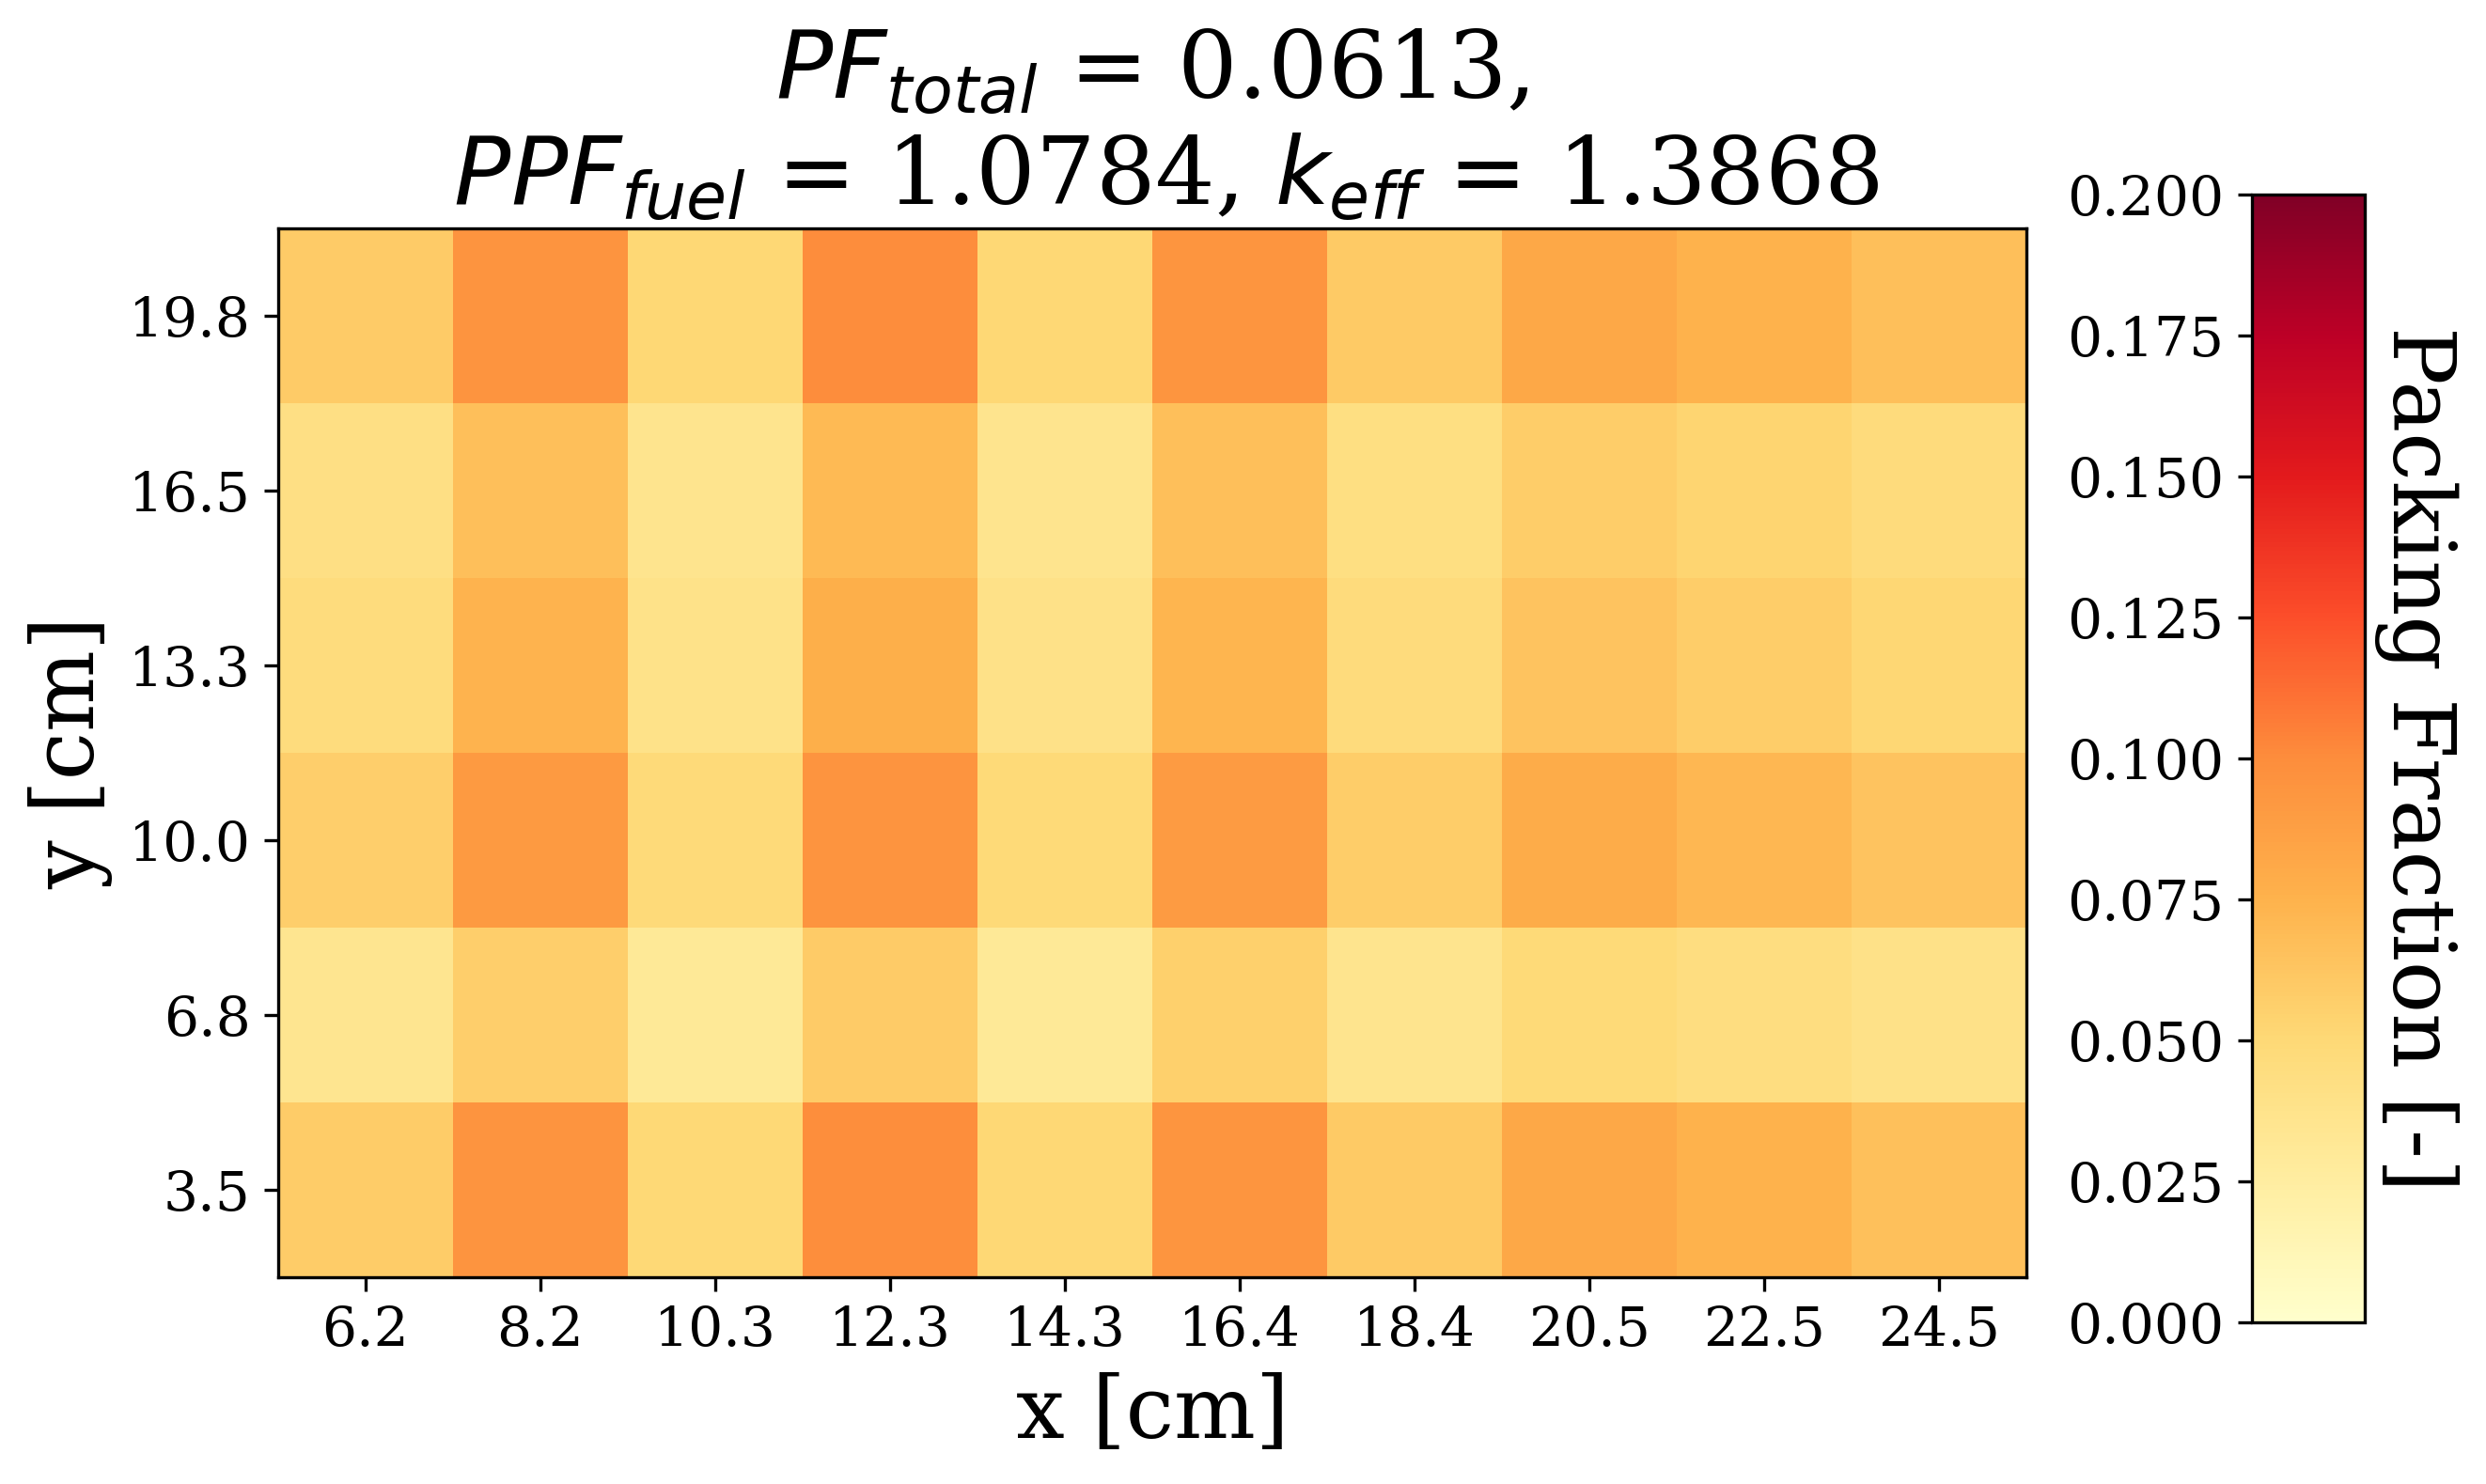
\includegraphics[width=0.49\linewidth]{a-3a-ppf-most-minimized.png} 
    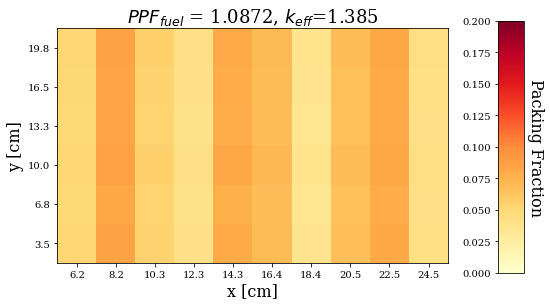
\includegraphics[width=0.49\linewidth]{a-1c-ppf-triso-comparison-most-minimized.png} 
    \caption{Simulation a-3a's most-minimized $PPF_{fuel}$ TRISO distribution 
    from Figure \ref{fig:assem-obj-3-most-minimized-distr} (left) and simulation a-1c's 
    most-minimized $PPF_{fuel}$ TRISO distribution from Figure 
    \ref{fig:assem-obj-1-ppf} (right).}
    \label{fig:a-3a-ppf-triso-comparison}
\end{figure}
Figure \ref{fig:a-3a-ppf-triso-comparison} shows that simulation a-3a's reactor model 1 
and simulation a-1a's most-minimized $PPF_{fuel}$ reactor model have similarly small 
packing fraction standard deviation of  $0.019$ and $0.017$, respectively. 
However, they do not follow the same TRISO distribution pattern, this could be 
attributed to the $PF_{total}$ and $PPF_{fuel}$ relationship resulting in unexpected 
TRISO distributions at different $PF_{total}$ values, as mentioned previously. 

Figure \ref{fig:a-3a-balanced-reactor-model} shows reactor model 22 which 
minimized $PF_{total}$, $T_{max}$, and $PPF_{fuel}$ to an equal extent by balancing 
influences from all objectives. 
\begin{figure}[htbp!]
    \centering
    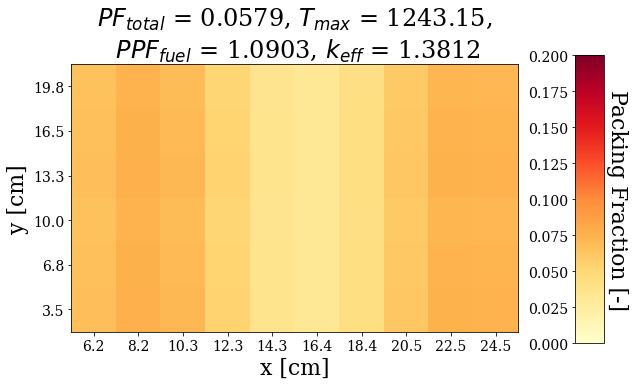
\includegraphics[width=0.6\linewidth]{a-3a-all-most-minimized.png} 
    \caption{Simulation a-3a's reactor model 22 which minimized $PF_{total}$, $T_{max}$, 
    and $PPF_{fuel}$ to an equal extent (see Pareto Front in 
    Figure \ref{fig:assem-obj-3-2d}).}
\label{fig:a-3a-balanced-reactor-model}
\end{figure}
% comment?

In all the reactor models on simulation a-3a's Pareto front (Figure 
\ref{fig:assem-obj-3-2d}), the TRISO distribution flatness is influenced by the 
minimize $T_{max}$ objective. 
The variations in \gls{TRISO} distributions are influenced by both the minimize 
$PF_{total}$ and minimize $PPF_{fuel}$ objectives. 
However, as mentioned previously, the $PF_{total}$ and $PPF_{fuel}$ relationship
results in unexpected TRISO distributions at different $PF_{total}$ values. 
The minimize $PF_{total}$ objective tries to maximize fission reaction rate
to enable a higher $k_{eff}$ for a lower $PF_{total}$, and 
the $PPF_{fuel}$ objective tries to flatten thermal flux. 

\subsubsection{Simulation a-3b}
In Section \ref{sec:a-3b}'s simulation a-3b, I conducted a three-objective 
optimization simulation to minimize total fuel packing fraction ($PF_{total}$), 
maximum temperature ($T_{max}$), and fuel-normalized power peaking factor 
($PPF_{fuel}$) in a one-third assembly model by varying $PF_{total}$, 
TRISO distribution, and coolant channel shape ($r_1, r_2, r_3, r_4, r_5$).
\gls{ROLLO} found 12 reactor models on simulation a-3b's Pareto 
front (Figure \ref{fig:assem-obj-3-all-2d}).

Compared to simulation a-3a in the previous section, simulation a-3b's reactor models 
have on average a lower $T_{max}$ value due to coolant channel shape variation. 
In simulation a-3b, \gls{ROLLO} found that the one-third assembly model with the 
most-minimized $PF_{total}$ objective, reactor model 11 (Figure 
\ref{fig:assem-obj-3-all-most-minimized-distr}), has an oscillating TRISO distribution 
along the x-axis and y-axis.
Figure \ref{fig:a-3a-pf-triso-comparison} compares simulation a-3b's reactor model 11 
and simulation a-1a's most-minimized $PF_{total}$ reactor model. 
\begin{figure}[htbp!]
    \centering
    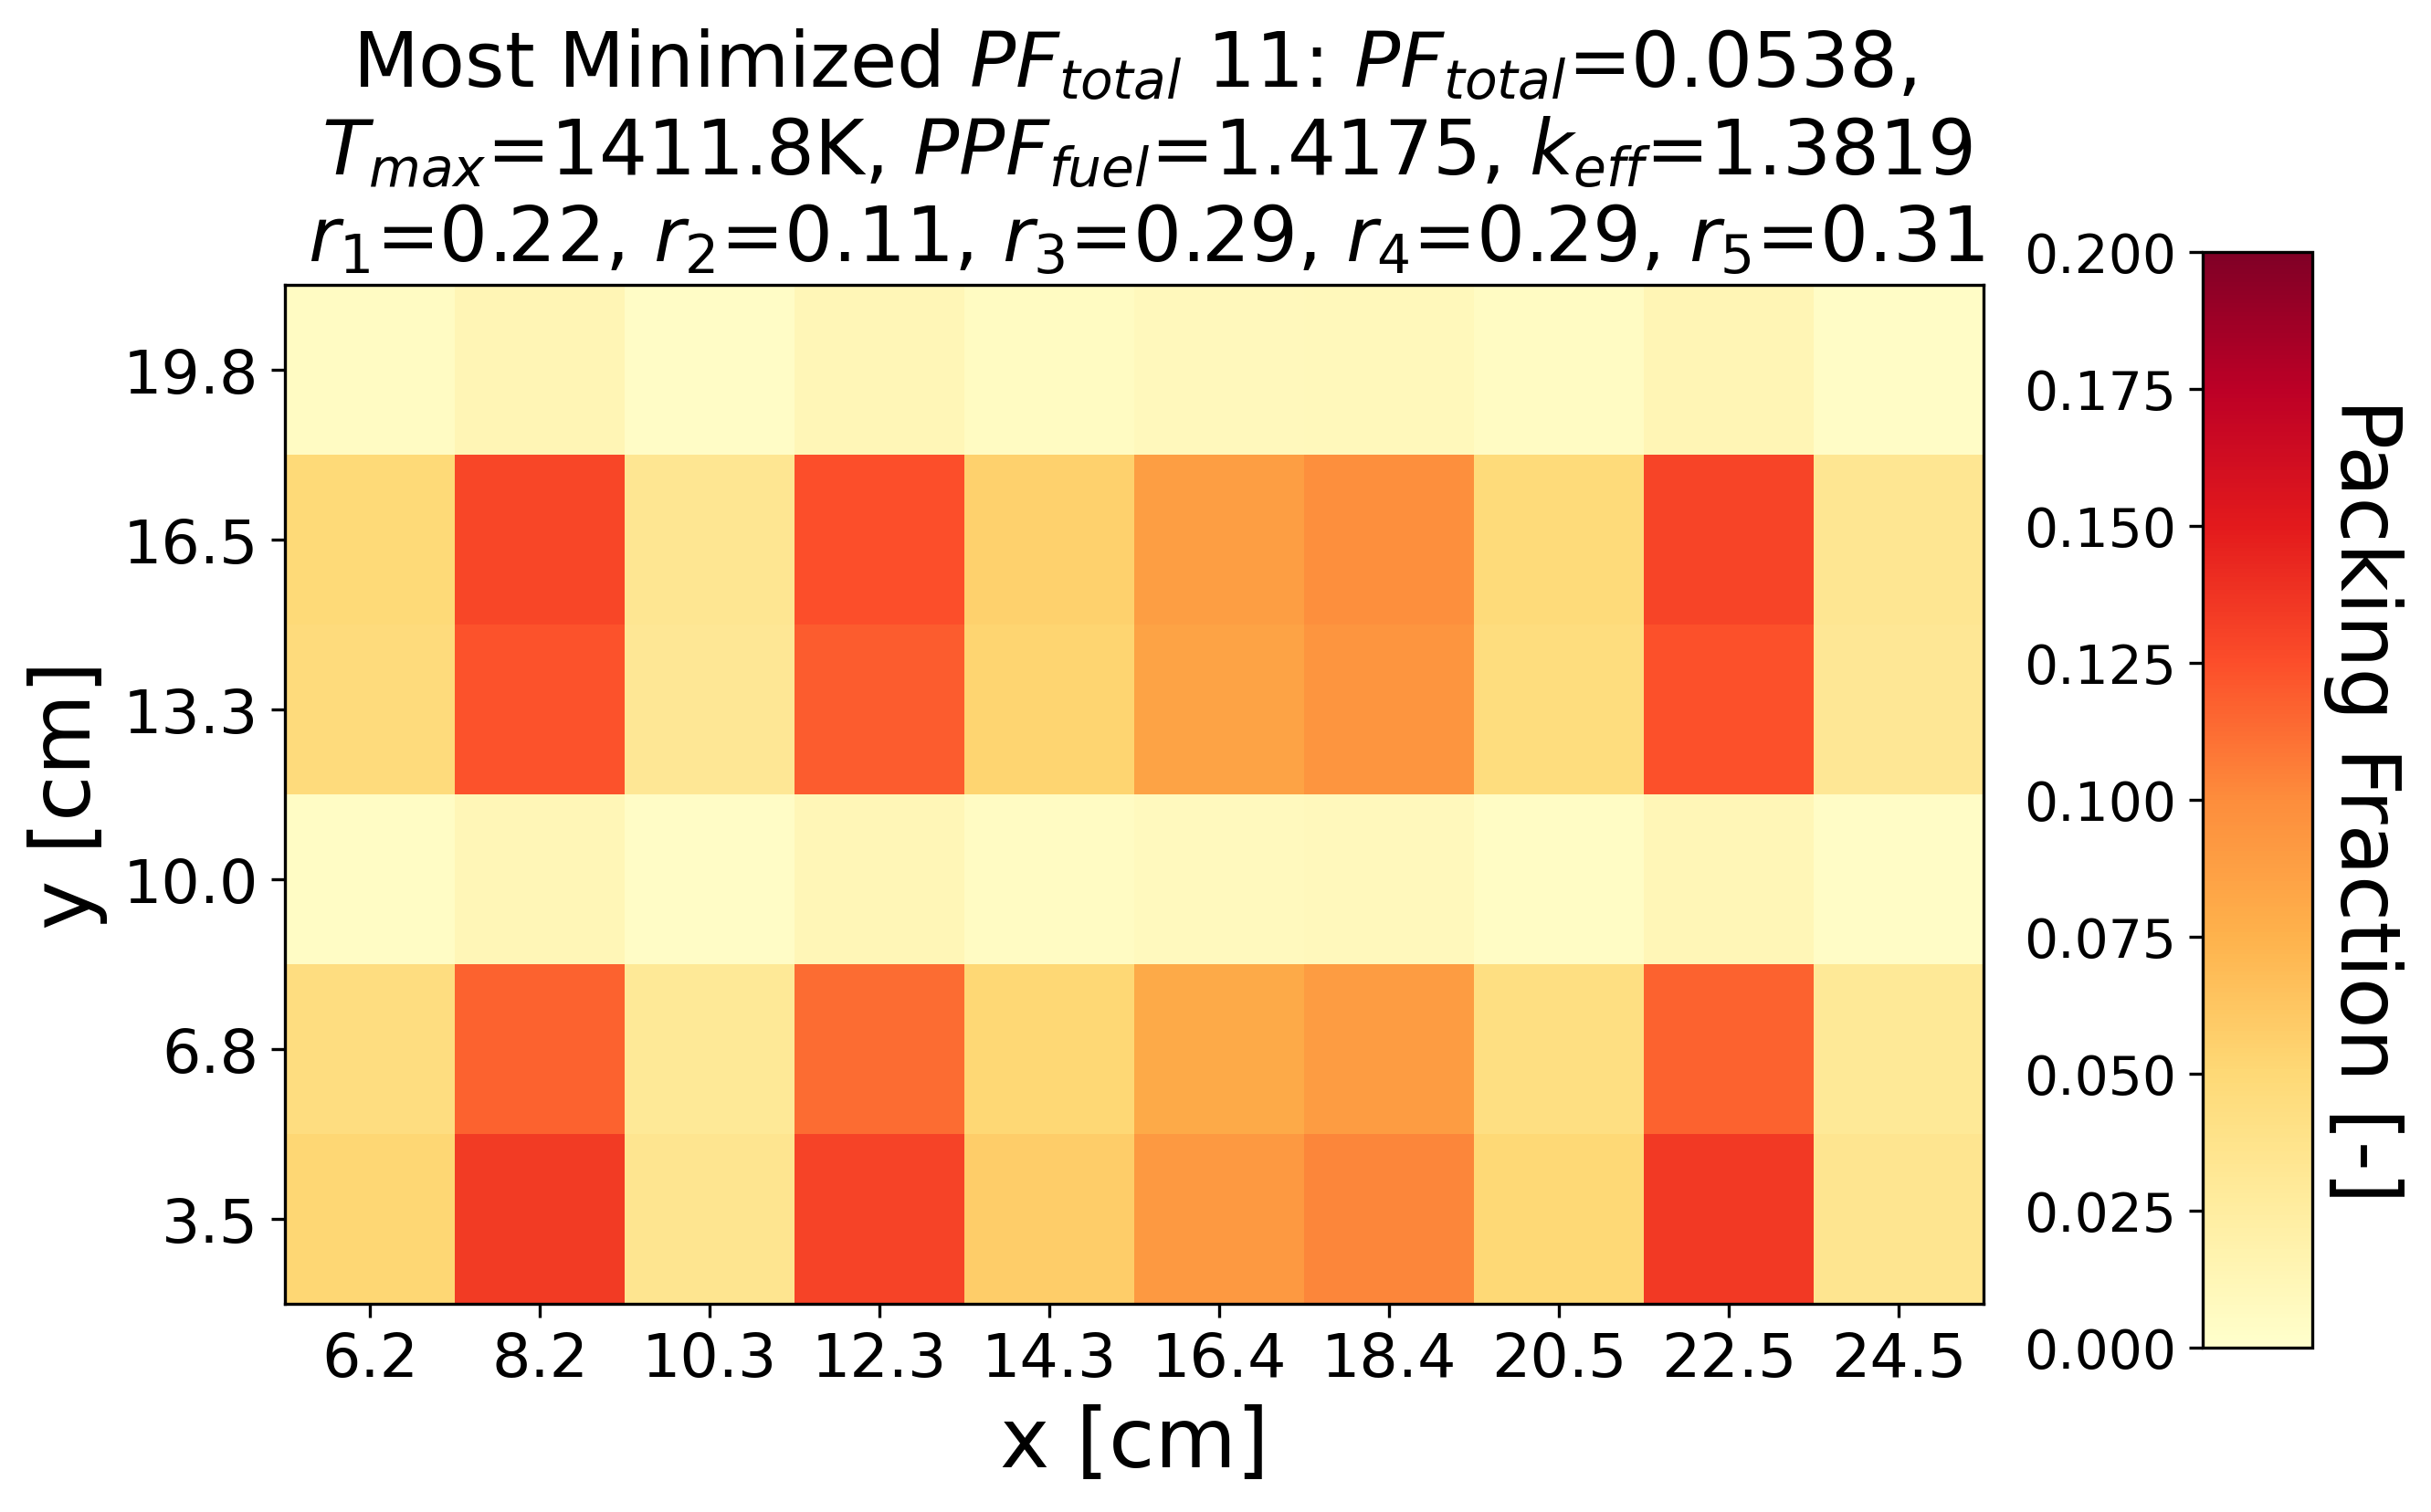
\includegraphics[width=0.49\linewidth]{a-3b-pf-most-minimized.png} 
    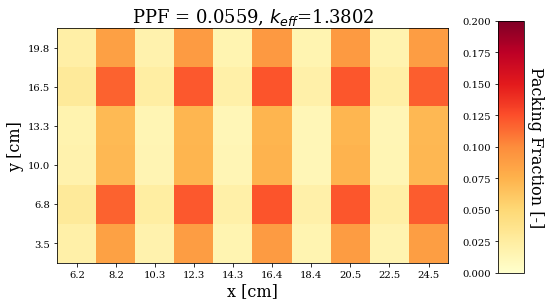
\includegraphics[width=0.49\linewidth]{assem-0.0559-most-minimized.png} 
    \caption{Simulation a-3b's most-minimized $PF_{total}$ TRISO distribution 
    from Figure \ref{fig:assem-obj-3-all-most-minimized} (left) and simulation a-1a's 
    most-minimized $PF_{total}$ TRISO distribution from Figure 
    \ref{fig:assem-obj-1-pf} (right).}
    \label{fig:a-3b-pf-triso-comparison}
\end{figure}
Figure \ref{fig:a-3b-pf-triso-comparison} shows that simulation a-3b's reactor model 11 
and simulation a-1a's most-minimized $PF_{total}$ reactor model have similarly large 
packing fraction standard deviation of $0.044$ and $0.04$, respectively. 
However, they do not follow the same TRISO distribution pattern, which is
attributed to the $PF_{total}$ and $PPF_{fuel}$ relationship resulting in unexpected 
TRISO distributions at different $PF_{total}$ values, as mentioned previously. 

In simulation a-3b, \gls{ROLLO} found that the one-third assembly model with the 
most-minimized $T_{max}$ objective, reactor model 1 (Figure 
\ref{fig:assem-obj-3-most-minimized-distr}), has an almost constant TRISO distribution.
Figure \ref{fig:a-3b-temp-triso-comparison} compares simulation a-3b's most-minimized 
$T_{max}$ reactor model 1 and simulation a-1b's most-minimized $T_{max}$ reactor model. 
\begin{figure}[htbp!]
    \centering
    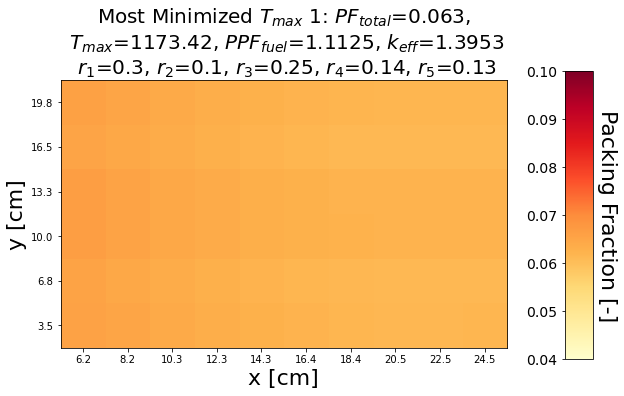
\includegraphics[width=0.49\linewidth]{a-3b-temp-most-minimized.png} 
    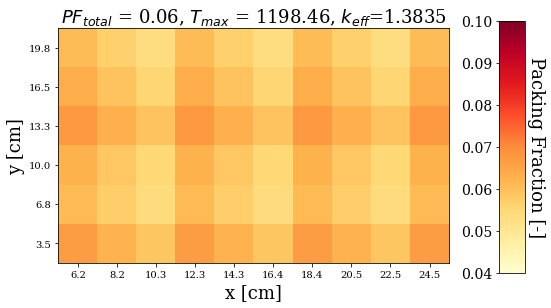
\includegraphics[width=0.49\linewidth]{a-1b-temp-most-minimized.png} 
    \caption{Simulation a-3b's most-minimized $T_{max}$ TRISO distribution 
    from Figure \ref{fig:assem-obj-3-most-minimized-distr} (left) and simulation a-1b's 
    most-minimized $T_{max}$ TRISO distribution from Figure 
    \ref{fig:assem-obj-1-temp} (right).}
    \label{fig:a-3b-temp-triso-comparison}
\end{figure}
Figure \ref{fig:a-3b-temp-triso-comparison} shows that simulation a-3b's most-minimized 
$T_{max}$ reactor model and simulation a-1b's most-minimized $T_{max}$ reactor model 
have similar almost constant TRISO distributions with packing fraction standard 
deviations of $0.001$ and $0.0009$, respectively.
However, they have different $PF_{total}$ values.

In simulation a-3b, \gls{ROLLO} found that the one-third assembly model with the 
most-minimized $PPF_{fuel}$ objective, reactor model 4 (Figure 
\ref{fig:assem-obj-3-all-most-minimized-distr}) has a slightly oscillating TRISO 
distribution along the y-axis.
Figure \ref{fig:a-3a-ppf-triso-comparison} compares simulation a-3b's most-minimized 
$PPF_{fuel}$ reactor model 4 and simulation a-1c's most-minimized $PPF_{fuel}$ reactor 
model. 
\begin{figure}[htbp!]
    \centering
    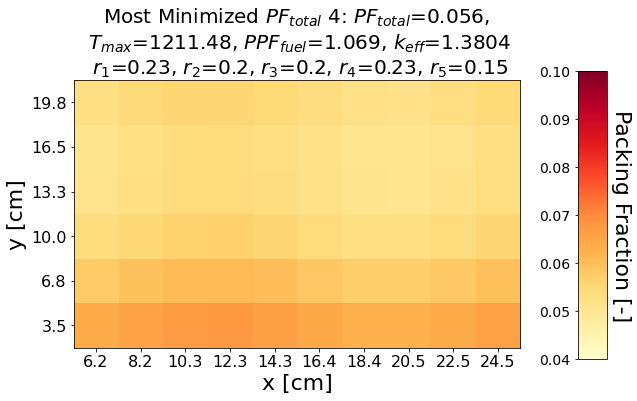
\includegraphics[width=0.49\linewidth]{a-3b-ppf-most-minimized.png} 
    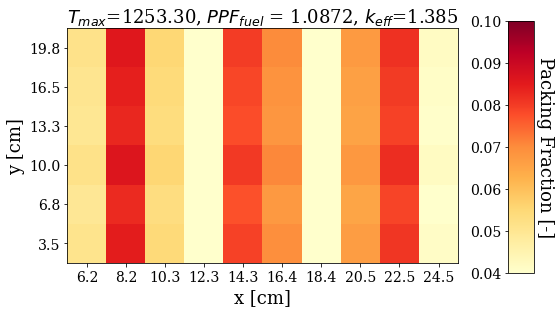
\includegraphics[width=0.49\linewidth]{a-1c-ppf-triso-comparison-most-minimized-01-scale.png} 
    \caption{Simulation a-3b's most-minimized $PPF_{fuel}$ TRISO distribution 
    from Figure \ref{fig:assem-obj-3-all-most-minimized-distr} (left) and simulation 
    a-1c's most-minimized $PPF_{fuel}$ TRISO distribution from Figure 
    \ref{fig:assem-obj-1-ppf} (right).}
    \label{fig:a-3b-ppf-triso-comparison}
\end{figure}
Figure \ref{fig:a-3b-ppf-triso-comparison} shows that simulation a-3b's reactor model 4 
and simulation a-1a's most-minimized $PPF_{fuel}$ reactor models both have small 
packing fraction standard deviation of  $0.005$ and $0.017$, respectively. 
However, they do not follow the same TRISO distribution pattern, this could be 
attributed to the $PF_{total}$ and $PPF_{fuel}$ relationship resulting in unexpected 
TRISO distributions at different $PF_{total}$ values, as mentioned previously.

Figure \ref{fig:a-3b-balanced-reactor-model} shows reactor model 2 which 
minimized $PF_{total}$, $T_{max}$, and $PPF_{fuel}$ to an equal extent by balancing 
influences from all objectives. 
\begin{figure}[htbp!]
    \centering
    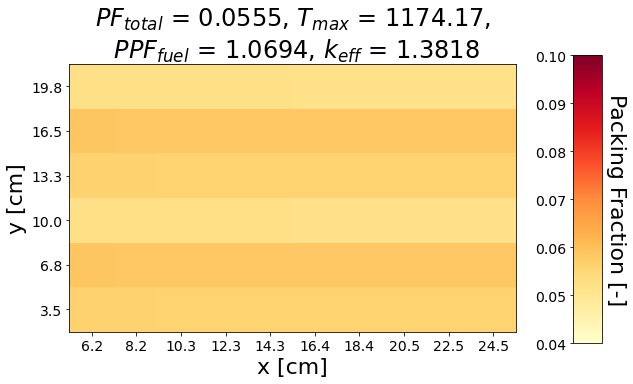
\includegraphics[width=0.6\linewidth]{a-3b-all-most-minimized.png} 
    \caption{Simulation a-3b's reactor model 2 which minimized $PF_{total}$, $T_{max}$, 
    and $PPF_{fuel}$ to an equal extent (see Pareto Front in 
    Figure \ref{fig:assem-obj-3-all-2d}).}
\label{fig:a-3b-balanced-reactor-model}
\end{figure}
Similar to simulation a-3a, for all the reactor models on simulation a-3b's Pareto front 
(Figure \ref{fig:assem-obj-3-all-2d}), the TRISO distribution flatness is influenced 
by the minimize $T_{max}$ objective. 
The variations in \gls{TRISO} distributions are influenced by both the minimize 
$PF_{total}$ and minimize $PPF_{fuel}$ objectives. 
However, as mentioned previously, the $PF_{total}$ and $PPF_{fuel}$ relationship
results in unexpected TRISO distributions at different $PF_{total}$ values. 
The minimize $PF_{total}$ objective tries to maximize fission reaction rate
to enable a higher $k_{eff}$ for a lower $PF_{total}$, and 
the $PPF_{fuel}$ objective tries to flatten thermal flux.

Figure \ref{fig:a-3b-centerline-temp} shows the one-third assembly centerline 
temperatures for three reactors on simulation a-3b's Pareto front: reactor model 11 
with most-minimized $PF_{total}$, reactor model 1 with most-minimized $T_{max}$, and
reactor model 4 with most-minimized $PPF_{fuel}$.
$r_1$, $r_2$, $r_3$, $r_4$, and $r_5$ values correspond to the FliBe channel at 18cm, 
15cm, 12cm, 8cm, and 6cm, respectively.  
\begin{figure}[htbp!]
    \begin{subfigure}{\textwidth}
        \centering
        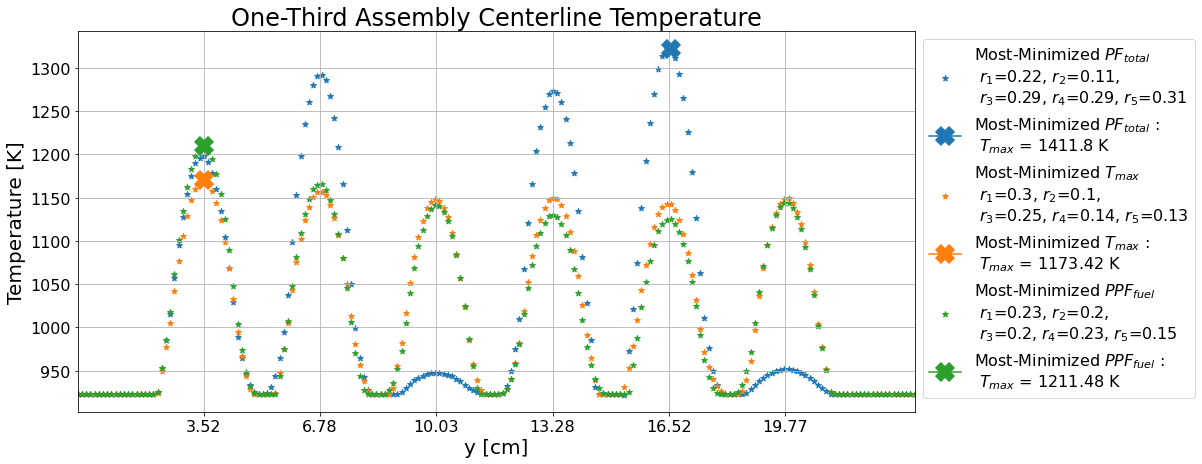
\includegraphics[width=\linewidth]{a-3b-centerline-temp.png}
        \caption{Centerline temperature. AHTR assembly's centerline is the white line 
        in Figure \ref{fig:ahtr-assem-verification}.}
        \label{fig:a-3b-centerline-temp} 
    \end{subfigure}
    \caption{Simulation a-3b's one-third assembly reactor models' temperature 
    distribution. Reactor models are on simulation a-3b's Pareto front: 
    reactor model 11 with most-minimized $PF_{total}$, 
    reactor model 1 with most-minimized $T_{max}$, and
    reactor model 4 with most-minimized $PPF_{fuel}$. 
    $r_1$, $r_2$, $r_3$, $r_4$, and $r_5$ values correspond to the FliBe channel at 18cm, 
    15cm, 12cm, 8cm, and 6cm, respectively.  }
    \label{fig:a-3b-temp-distribution}
\end{figure}
Section \ref{sec:assem-discussion-temp} concluded that the one-third assembly's FLiBe 
channels (corresponding to $r_1, r_2, r_3, r_4, r_5$) closest to the temperature peaks 
are most important to minimizing $T_{max}$, however, coolant channel shape variation 
does not have as high of an impact on $T_{max}$ as \gls{TRISO} distribution variation: 
the average $T_{max}$ due to \gls{TRISO} variation decreased by $\sim150K$ over 3 
generations, while average $T_{max}$ due to coolant channel shape variation only 
decreased by $\sim10K$ over 3 generations. 
Sections \ref{sec:assem-discussion-pf}, \ref{sec:assem-discussion-temp}, and 
\ref{sec:assem-discussion-ppf} also concluded that only coolant channel shape is only 
correlated with the minimize $T_{max}$ objective. 

Figure \ref{fig:a-3b-centerline-temp} shows that reactor model 11 with most minimized 
$PF_{total}$ peaks in the 4th graphite plank (at 16.52cm) and has $r_1 = 0.22cm$ and 
$r_2 = 0.11cm$, reactor model 1 with most minimized $T_{max}$ peaks in the 1st 
graphite plank (at 3.52cm) and has $r_5 = 0.13cm$, and reactor model 4 with most 
minimized $PPF_{fuel}$ peaks in the 1st graphite plank (at 3.52cm) and has 
$r_5 = 0.15cm$. 
All their radius values are unexpectedly small. 
This could be due to coolant channel shape not having a high impact on $T_{max}$ compared 
to TRISO distribution, thus \gls{ROLLO} was more influenced by TRISO distribution when 
searching for optimal reactor models. 
This paired with simulation a-3b's 128 individuals per generation possibly being  
too small to explore reactor models with 12 input parameters. 
Simulation a-3b has 12 input parameters which is higher than all the other optimization 
simulations which have 7 or less input parameters. 
A larger population size will enable \gls{ROLLO} to explore more reactor model variation, 
and potentially find even more optimal reactor models. 
To better explore simulation a-3b's design space, I re-run simulation a-3b with 
256 individuals per generation. 

\subsubsection{Simulation a-3b with 256 Population Size}
Simulation a-3b-256 has the exact same optimization problem parameters as simulation 
a-3b (Table \ref{tab:simulationa3b}) except for an increase in population size to 256
individuals. 
Figure \ref{fig:assem-obj-3-all-256-2d} shows a plot of the final generation's reactor 
models' $PF_{total}$ against $T_{max}$ against $PPF_{fuel}$; crosses mark the reactor 
models that fall on the Pareto front.
Figure \ref{fig:assem-obj-3-all-256-distr} shows the 38 TRISO packing fraction 
distributions in the final generation that fall on the Pareto front. 
\begin{figure}[htbp!]
    \begin{subfigure}{\textwidth}
        \centering
        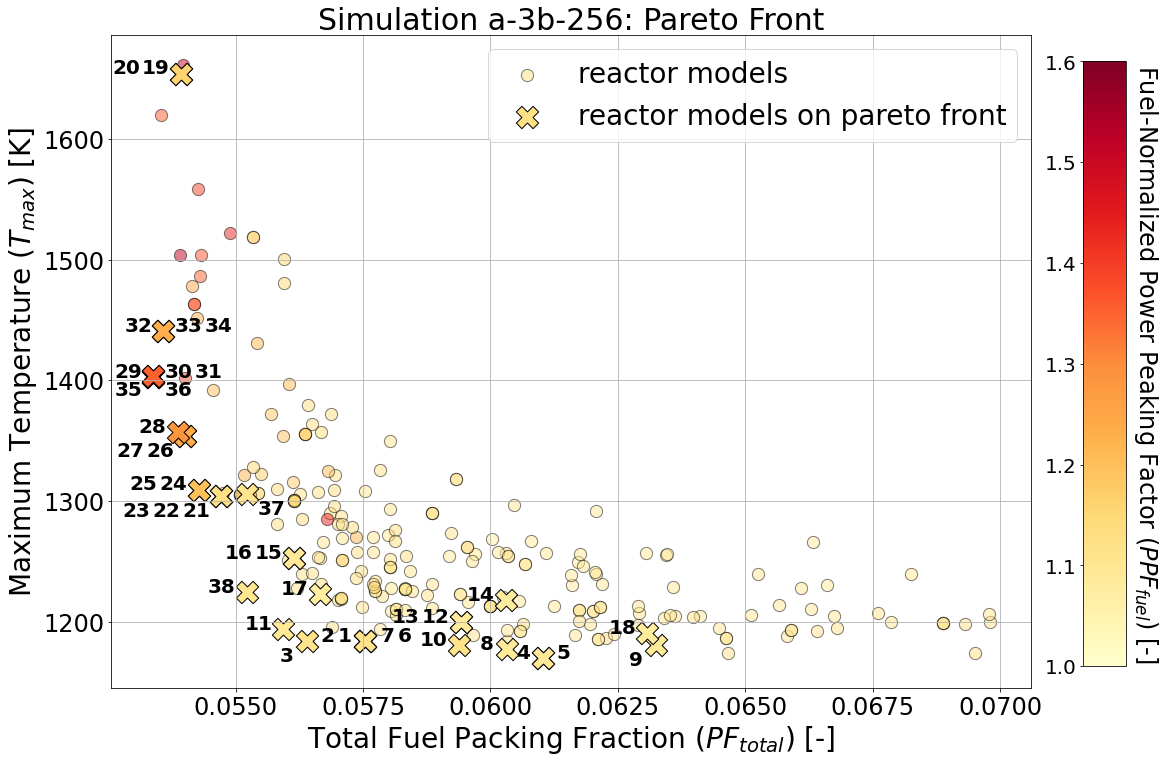
\includegraphics[width=\linewidth]{assem-obj-3-all-256-2d.png}
        \caption{Plot of final generation's reactor models' $PF_{total}$ against 
        $T_{max}$ against $PPF_{fuel}$ as a color dimension. 
        Crosses indicate the reactor models on the 
        Pareto front. Cross numbering correspond to TRISO distributions in Figure 
        \ref{fig:assem-obj-3-all-distr}.}
        \label{fig:assem-obj-3-all-256-2d} 
    \end{subfigure}
    \caption{Simulation a-3b-256 -- ROLLO three-objective optimization with 
    256 population size to minimize total fuel packing fraction ($PF_{total}$), 
    maximum temperature ($T_{max}$), and fuel-normalized power peaking factor 
    ($PPF_{fuel}$) in the one-third assembly. 
    Input parameters varied: total fuel packing fraction $PF_{total}$, 
    TRISO packing fraction distribution ($\rho_{TRISO}(\vec{r})$), 
    coolant channel shape $(r_1, r_2, r_3, r_4, r_5)$.}
    \label{fig:assem-obj-3-all-256}
\end{figure}
\begin{figure}[htbp!]
    \ContinuedFloat
    \begin{subfigure}{\textwidth}
        \centering
        \includegraphics[width=\linewidth]{assem-obj-3-all-256-distr.png}
        \caption{TRISO distributions for the 38 reactor models on the Pareto front.
        Numbered reactor models correspond to numbered crosses in Figure 
        \ref{fig:assem-obj-3-all-256-2d}. }
        \label{fig:assem-obj-3-all-256-distr} 
    \end{subfigure}
    \caption{(contd.) Simulation a-3b-256 -- ROLLO three-objective optimization with 
    256 population size to minimize total fuel packing fraction ($PF_{total}$), 
    maximum temperature ($T_{max}$), and fuel-normalized power peaking factor 
    ($PPF_{fuel}$) in the one-third assembly. 
    Input parameters varied: total fuel packing fraction $PF_{total}$, 
    TRISO packing fraction distribution ($\rho_{TRISO}(\vec{r})$), 
    coolant channel shape $(r_1, r_2, r_3, r_4, r_5)$.}
\end{figure}

Figure \ref{fig:assem-obj-3-all-256} demonstrates that \gls{ROLLO} found 38 reactor 
models on simulation a-3b-256 final generation's Pareto front. 
Figure \ref{fig:assem-obj-3-all-256-most-minimized} shows three reactor models on the 
Pareto front that most-minimized each objective, and one reactor model on the 
Pareto front that equally minimized all three objectives. 
I selected the equally minimized reactor model by visually studying Figure 
\ref{fig:assem-obj-3-all-256} and selecting a reactor model that is close to the origin 
and has a light yellow color dimension. 
Reactor model 36 most-minimized $PF_{total}$, reactor model 4 most-minimized $T_{max}$, 
reactor model 17 most-minimized $PPF_{fuel}$, and reactor model 11 equally minimized 
all three objectives. 
\begin{figure}[htbp!]
    \centering
    \begin{subfigure}{\textwidth}
    \centering
    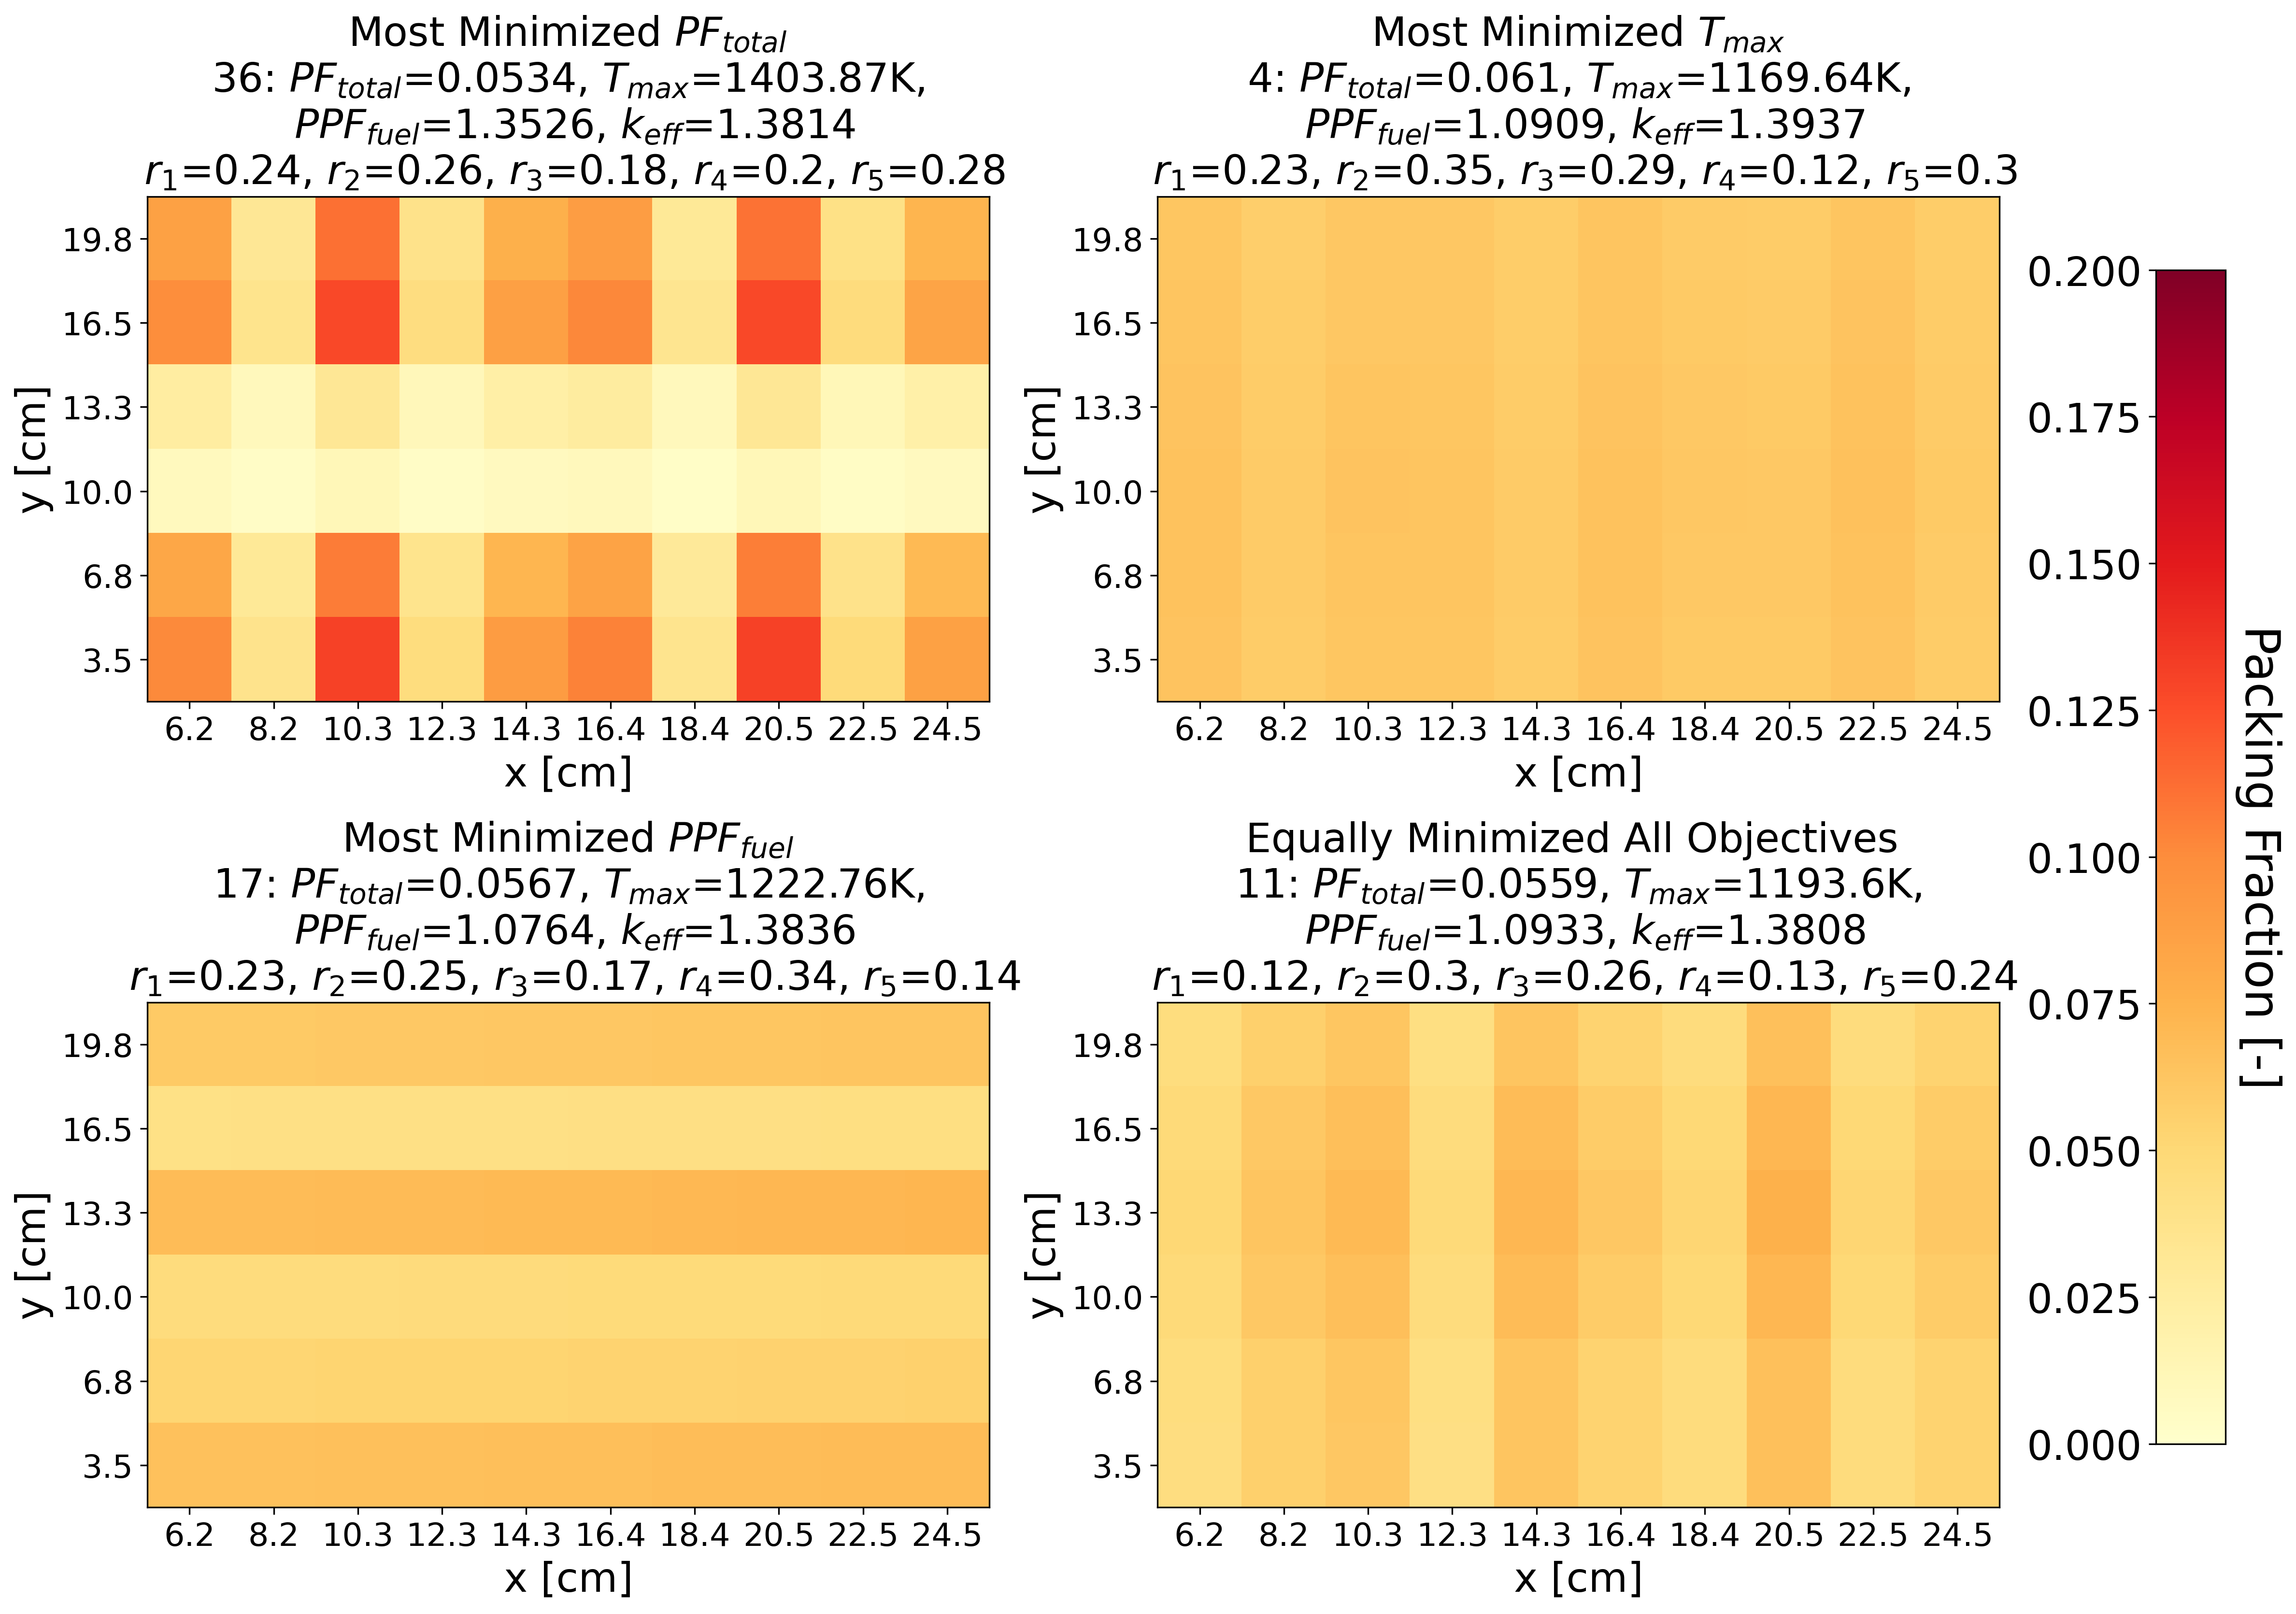
\includegraphics[width=\linewidth]{assem-obj-3-all-256-distr-most-minimized.png}
    \caption{TRISO packing fraction distributions.}
    \label{fig:assem-obj-3-all-256-most-minimized-distr}
    \end{subfigure}
    \caption{AHTR one-third assembly models and TRISO distributions for the 3 reactor 
    models on simulation a-3b-256's Pareto front that most-minimized each objective, and 
    1 reactor model that equally minimized all three objectives.
    Simulation a-3b -- ROLLO three-objective optimization to minimize 
    total fuel packing fraction ($PF_{total}$), maximum temperature ($T_{max}$), 
    and fuel-normalized power peaking factor ($PPF_{fuel}$) in the one-third assembly. 
    Input parameters varied: total fuel packing fraction $PF_{total}$, 
    TRISO packing fraction distribution ($\rho_{TRISO}(\vec{r})$), 
    coolant channel shape $(r_1, r_2, r_3, r_4, r_5)$.}
    \label{fig:assem-obj-3-all-256-most-minimized}
\end{figure}

Figure \ref{fig:a-3b-256-temp-distribution} shows the one-third assembly centerline 
temperatures for three reactors on simulation a-3b-356's Pareto front: reactor model 36 
with most-minimized $PF_{total}$, reactor model 4 with most-minimized $T_{max}$, and
reactor model 17 with most-minimized $PPF_{fuel}$.
$r_1$, $r_2$, $r_3$, $r_4$, and $r_5$ values correspond to the FliBe channel at 18cm, 
15cm, 12cm, 8cm, and 6cm, respectively.  
\begin{figure}[htbp!]
    \begin{subfigure}{\textwidth}
        \centering
        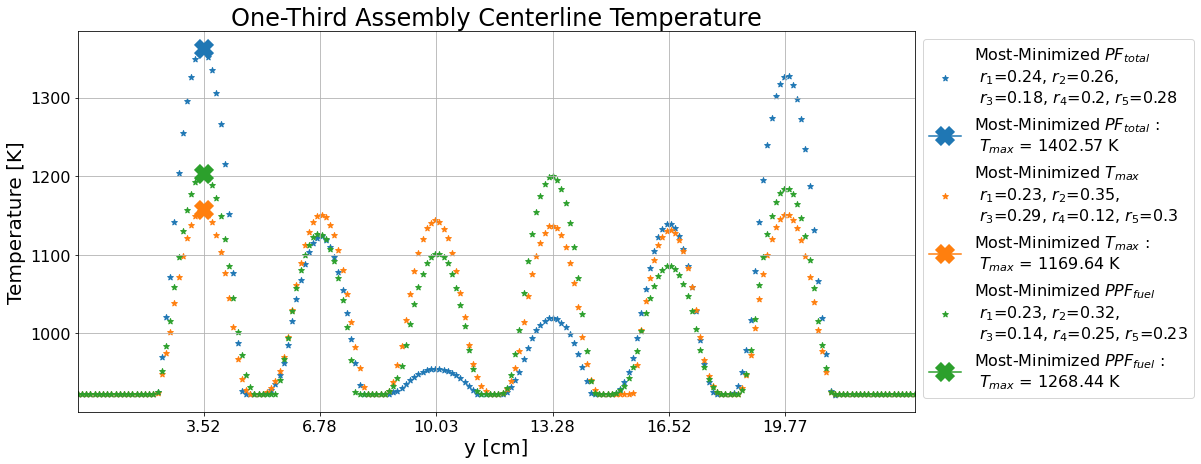
\includegraphics[width=\linewidth]{a-3b-256-centerline-temp.png}
        \caption{Centerline temperature. AHTR assembly's centerline is the white line 
        in Figure \ref{fig:ahtr-assem-verification}.}
        \label{fig:a-3b-256-centerline-temp} 
    \end{subfigure}
    \caption{Simulation a-3b-256's one-third assembly reactor models' temperature 
    distribution. Reactor models are on simulation a-3b-256's Pareto front: 
    reactor model 36 with most-minimized $PF_{total}$, 
    reactor model 4 with most-minimized $T_{max}$, and
    reactor model 17 with most-minimized $PPF_{fuel}$.
    $r_1$, $r_2$, $r_3$, $r_4$, and $r_5$ values correspond to the FliBe channel at 18cm, 
    15cm, 12cm, 8cm, and 6cm, respectively.  }
    \label{fig:a-3b-256-temp-distribution}
\end{figure}
Figure \ref{fig:a-3b-256-centerline-temp} shows that all three reactor models 
peak in the 1st graphite plank (at 3.52cm) with $r_1$ values of $\sim0.23cm$. 
The larger radius values closer to temperature peaks enables lower $T_{max}$ values, 
in simulation a-3b-256 compared to simulation a-3b's equivalent reactor models 
(Figure \ref{fig:a-3b-centerline-temp}). 
This suggests that simulation a-3b-256's larger population size enabled \gls{ROLLO} 
to explore more reactor model variation, and find even more optimal reactor models 
that further minimized $T_{max}$. 

\pagebreak
\section{Summary}
\glsresetall
This chapter described the \gls{AHTR} one-third assembly's \gls{ROLLO} optimization 
results. 
I varied the following \gls{AHTR} one-third assembly input parameters: \gls{TRISO} 
packing fraction distribution ($\rho_{TRISO}(\vec{r})$), total fuel packing fraction 
($PF_{total}$), and coolant channel shape; in an effort to minimize the following 
objectives: $PF_{total}$, maximum temperature ($T_{max}$), and fuel-normalized power 
peaking factor ($PPF_{fuel}$) in the one-third assembly. 

In Section \ref{sec:assem-one-obj}'s single-objective optimization simulations: 
a-1a, a-1b, a-1c, a-1d, a-1e, a-1f; and Sections \ref{sec:assem-discussion-pf}, 
\ref{sec:assem-discussion-temp}, and \ref{sec:assem-discussion-ppf} discussions,    
I verified that each of the one-third assembly objective follows the same driving 
factors as the \gls{AHTR} plank optimization objectives (Chapter 
\ref{chap:ahtr-plank-opt-results}) and described each objective's relationship with 
each input parameter. 
I determined that the minimize $T_{max}$ objective is driven by minimizing one-third 
assembly's maximum temperature; and flattens TRISO distribution and maximizes 
the FLiBe channels radius values ($r_1, r_2, r_3, r_4, r_5$) that are close 
to the reactor model's temperature peak to achieve the objective. 
The minimize $PF_{total}$ objective is driven by maximizing the one-third assembly's 
total fission reaction rate and influences oscillations in the TRISO disribution to 
achieve the objective. 
The minimize $PPF_{fuel}$ objective is driven by flattening the one-third assembly's 
thermal flux distribution and influences $PF_{total}$ and oscillations in the TRISO 
disribution to achieve the objective. 
Both the minimize $PF_{total}$ and minimize $PPF_{fuel}$ objectives have no correlation 
with the coolant channel shape. 

In Sections \ref{sec:assem-two-obj} and \ref{sec:assem-three-obj}'s multi-objective 
optimization simulations: a-2a, a-2b, a-2c, a-3a, a-3b, and a-3b-256; and Section 
\ref{sec:assem-discussion-multi}'s discussions, I further analyzed how the objectives' 
combined effects resulted in the optimal reactor models found by each multi-objective 
optimization simulation. 
All the multi-objective optimization simulations successfully found a wide spread of 
reactor models on their Pareto fronts that meets each objective to varying degrees. 
In the multi-objective optimization simulations, the minimize $T_{max}$ objective 
continued to influence the flattening of the TRISO distribution and maximizing of 
the FLiBe channels radius values ($r_1, r_2, r_3, r_4, r_5$) that are close 
to the reactor model's temperature peak. 
The results from simulation a-2b suggested that the minimize $PF_{total}$ 
objective's driving factor maximize total fission reaction rate and 
minimize $PPF_{fuel}$ objective's driving factor flattening thermal flux distribution 
influence each other resulting in unexpected TRISO distributions at different 
$PF_{total}$ values. 

Simulation a-3b-256's multi-objective optimization shows the result of minimizing all 
three objectives (minimize $PF_{total}$, $T_{max}$, and $PPF_{fuel}$) while varying 
all the input parameters ($PF_{total}$, TRISO distribution, and coolant channel shape).
Figure \ref{fig:assem-obj-3-all-256} shows the 38 reactor models on simulation 
a-3b-256's Pareto front that meet the three objectives to varying degrees. 
The reactor models on the Pareto Front have different TRISO distributions and coolant
channel shapes, depending on the extent each objective is minimized. 

This chapter demonstrated \gls{ROLLO}'s success in conducting multi-objective 
optimization, a global search of the large reactor design space, to find optimal reactor 
models on the Pareto front that satisfy all the objectives. 
Reactor designers can utilize \gls{ROLLO} for multi-objective optimization problems with 
any number of objectives and arbitrary input parameters, to narrow down the search space 
to find reactor models that meet their desired requirements. 
The results from \gls{ROLLO}'s multi-objective optimizations help reactor designers 
gain a clearer understanding of the reactor models' parameters that meet their defined 
objectives to varying degrees.
From there, reactor designers can determine the importance of each objective for 
their purposes, then conduct sensitivity analysis and use higher fidelity models to 
further study a smaller section of the optimal design space that they are 
interested in.

% talk about a-3b result, what is recommended for the AHTR assembly's geometry. 